\documentclass[11pt,a4paper,oneside]{book}
%-- coding: UTF-8 --
\usepackage[UTF8]{ctex}
\usepackage{fontspec}
\defaultfontfeatures{Mapping=tex-text}
\usepackage{xunicode}%防止pdf乱码
%\usepackage{ccmap}%
\usepackage{xltxtra}
\usepackage{amsmath}
\usepackage{amsfonts}
\usepackage{amssymb}
\usepackage{graphicx}
\usepackage{amsthm}
\usepackage{array}
\usepackage{float}   %{H}
\usepackage{booktabs}  %\toprule[1.5pt]
\setcounter{secnumdepth}{4}
\usepackage{indentfirst} %首行缩进
\usepackage{tcolorbox} %彩色框框
\usepackage{graphicx}  %图片并排
\usepackage{subfigure} %图片并排
\usepackage{graphicx} %插入jpg
\usepackage[toc]{multitoc} %双列目录
\setcounter{secnumdepth}{4}		%增加编号深度
\setcounter{tocdepth}{4}		%增加目录深度
\usepackage{hyperref}     %生成pdf书签
\hypersetup{hidelinks,
	colorlinks=true,
	allcolors=black,
	pdfstartview=Fit,
	breaklinks=true
}       %去掉目录的红色框框
%===================%插入代码需要的控制
\usepackage{listings}
\usepackage{xcolor}
\setmonofont{Consolas}%字体
\lstset{%
	numbers=left,
	numberstyle=\tt\tiny,%
	showstringspaces=false,
	showspaces=false,%
	tabsize=4,%
	frame=lines,%
	basicstyle=\tt\small,%
	keywordstyle=\color{ blue!70}\bfseries,%
	identifierstyle=,%
	commentstyle=\color{red!50!green!50!blue!50},%\itshape,%
	stringstyle=\color{black},%
	breaklines=true
}
%===================%
\usepackage[left=2cm,right=2cm,top=2cm,bottom=2cm]{geometry}
\newtheorem{theorem}{定理}
\newtheorem{definition}{定义}
\newtheorem{e}{例}
\title{\Huge Circuit Analysis}
\author{严中圣}
\date{\today}

\begin{document}
\maketitle
\tableofcontents  %目录
\chapter{电路模型和电路定律}
\section{电路和电路模型}
\textbf{概念定义:}
\begin{enumerate}
	\item 实际电路:由电工设备和电气器件按预期目的连接构成的电流的通路。
	
	功能:
	\begin{enumerate}
		\item 能量的传输、分配与转换
		\item 信息的传递、控制与处理
	\end{enumerate}
	\item 电路模型:反映实际电路部件的\textbf{主要电磁
	性质}的理想电路元件及其组合。
	\item 理想电路元件:
	有某种确定的电磁性能并有精确的数学定义的基本结构。
	\item 5种基本的理想电路元件:
	\begin{enumerate}
		\item 电阻元件:表示消耗电能的元件
		\item 电感元件:表示产生磁场,储存磁场能量的元件
		\item 电容元件:表示产生电场,储存电场能量的元件
		\item 电压源和电流源:表示将其它形式的能量转变成
		电能的元件。
	\end{enumerate}	
\end{enumerate}
\noindent \textbf{注意:}
\begin{enumerate}
	\item[(1)]五种基本理想电路元件有三个特征:
	\begin{enumerate}
		\item 只有两个端子;
		\item 可以用电压或电流按数学方式描述;
		\item 不能被分解为其他元件。
	\end{enumerate}
	\item[(2)] 具有相同的主要电磁性能的实际电路部件,在一定条件下可用同一电路模型表示;
	同一实际电路部件在不同的应用条件下,其电路模型可以有不同的形式。
\end{enumerate}
\section{电流和电压的参考方向}
\subsection{电流的参考方向}
电流:带电粒子有规则的定向运动

电流强度:单位时间内通过导体横截面的电荷量
\begin{equation}
	i(t)=\lim_{\Delta t \rightarrow 0} \frac{\Delta q}{\Delta t}=\frac{dq}{dt}
\end{equation}
参考方向:任意假定一个正电荷运动的方向即为电流的参考方向。

电流的参考方向与实际方向的关系:
\begin{figure}[H]
	\centering
	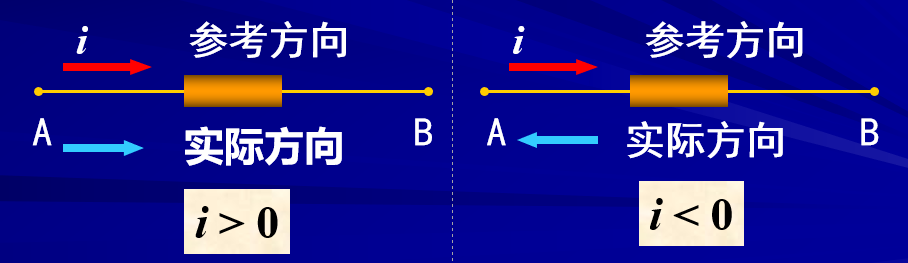
\includegraphics[width=0.7\linewidth]{screenshot107}
	\caption{电流的参考方向与实际方向的关系}
	\label{fig:screenshot107}
\end{figure}
\subsection{电压的参考方向}
电位$\varphi$:单位正电荷$q$从电路中一点移至参考点($\varphi=0$)时电场力做功的大小。

电压:单位正电荷$q$从电路中一点移至另一点时电场力做功($W$)的大小。
\begin{equation}
	U=\frac{dW}{dq}
\end{equation}
实际电压方向:电位真正降低的方向。
\begin{figure}[H]
	\centering
	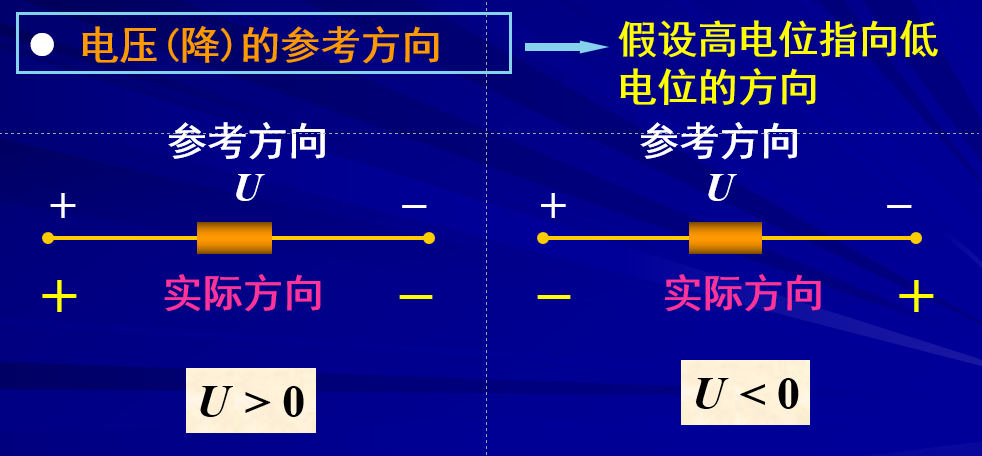
\includegraphics[width=0.7\linewidth]{screenshot108}
	\caption{电压的参考方向与实际方向的关系}
	\label{fig:screenshot108}
\end{figure}
\subsection{关联参考方向}
元件或支路的$u,i$采用相同的参考方向称之为关联参考方向。反之,称为非关联参考方向。
\begin{figure}[H]
	\centering
	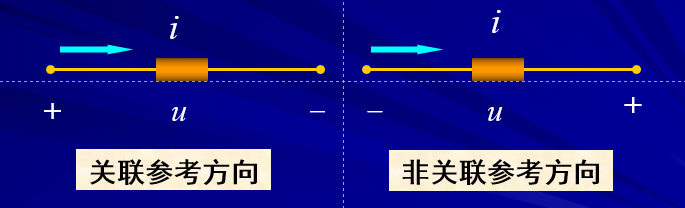
\includegraphics[width=0.7\linewidth]{screenshot109}
	\caption{关联参考方向示意图}
	\label{fig:screenshot109}
\end{figure}

\section{电功率和能量}
电功率:单位时间内电场力所做的功。
\begin{equation}
	p=\frac{dW}{dt}=\frac{dW}{dq} \frac{dq}{dt}=ui
\end{equation}
\textbf{电路吸收或发出功率的判断}:
\begin{figure}[H]
	\centering
	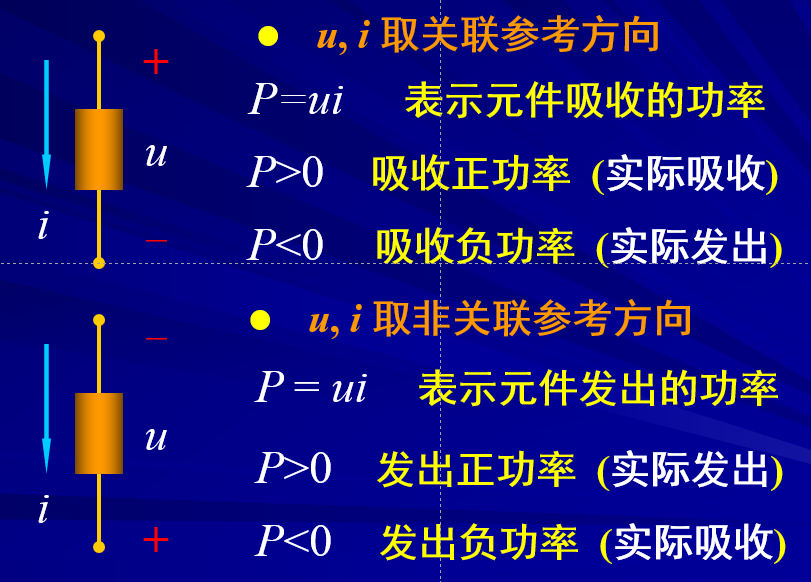
\includegraphics[width=0.7\linewidth]{screenshot110}
	\caption{电路吸收或发出功率判断示意图}
	\label{fig:screenshot110}
\end{figure}
\textbf{注意:}
对一完整的电路,满足:发出的功率=吸收的功率
\section{电路元件}
\subsection{电路元件}
电路元件:是电路中最基本的组成单元。

\textbf{注意:}如果表征元件端子特性的数学关系式是线性关系,该元件称为\textbf{线性元件},否则称为\textbf{非线性元件}。

\textbf{思考:}电阻、电感与电容是线性元件还是非线性元件?

线性元件:是一种电子元件,在电子电路中与电流或电压有线性的关系。
电阻是最普遍的线性元件范例,常见的线性元件还有电容和电感。线性元件是指输出量和输入量具有正比关系的元件。例如在温度不变的情况下金属电阻元件的两端电压同电流的关系就可以认为是线性的。金属导体、电解液也都具有这一特性。电子元器件具有这种关系的很多。质量差的元器件在一定情况下会出现“线性失真”,就是在这样的情况下输入量和输出量不再满足线性关系了。[来自百度百科]

对于线性元件,其满足齐次性和可加性。线性元件可以用一次线性代数式,也可以是线性的微分或积分形式。
\begin{enumerate}
	\item[(1)]电阻
	
	线性电阻满足:
	\begin{equation}
		R=\frac{U}{I}
	\end{equation}
	\item[(2)]电感
	
	电感(Inductance)是闭合回路的一种属性,即当通过闭合回路的电流改变时,会出现电动势来抵抗电流的改变。如果这种现象出现在自身回路中,那么这种电感称为自感(self-inductance),是闭合回路自己本身的属性。假设一个闭合回路的电流改变,由于感应作用在另外一个闭合回路中产生电动势,这种电感称为互感(mutual inductance)。电感元件是一种储能元件,电感元件的原始模型为导线绕成圆柱线圈。当线圈中通以电流$i$,在线圈中就会产生磁通量$\phi$,并储存能量。电感以方程表达为
	\begin{equation}
		\varepsilon=-L\frac{di}{dt}
	\end{equation}
	\begin{enumerate}
		\item 判断齐次性:
		\begin{equation}
			\mbox{若取}\varepsilon_2=2\varepsilon_1,\mbox{则}i_2=L\frac{d\varepsilon_2}{dt}=L\frac{d(2\varepsilon_1)}{dt}=2i_1
		\end{equation}
		\item 判断可加性:
		\begin{equation}
			\mbox{若取}\varepsilon=\varepsilon_1+\varepsilon_2\mbox{,则}i=L\frac{d(\varepsilon1+\varepsilon2)}{dt}=i_1+i_2
		\end{equation}
		
	\end{enumerate}
	\item[(3)]电容
	
	电容元件的定义:如果一个二端元件在任一时刻,其电荷与电压之间的关系由$u-q$平面上一条曲线所确定,则称此二端元件为电容元件。通过坐标原点一条直线的电容元件称为线性电容元件,否则称为非线性电容元件。
	
	线性电容的电流与电压满足:
	\begin{equation}
		i=\frac{dq}{dt}=C\frac{du}{dt}
	\end{equation}
	齐次性和可加性可同上判断。
\end{enumerate}
普通的电感和电容在常规工作范围内,属于线性元件.也就是说,他的阻抗基本上与输入的电压或者电流无关. 特殊的电感、电容甚至电阻或有非线性的,例如:饱和电抗器,饱和调压器的电抗电感,压敏电阻等.属于非线性元件.非线性元器件的显著特点,就是阻抗随输入电压(或者电流)的变化而变化.
\subsection{集总参数电路}
定义:由集总元件构成的电路\par 集总元件:假定发生的电磁过程都集中在元件内部进行。\par 集总条件:$d<<\lambda$

集总参数电路中$u、i$可以是时间的函数,但与空间坐标无关。因此,任何时刻,流入两端元件一个端子的电流等于从另一端子流出的电流;端子间的电压为单值量。

\section{电阻元件}
定义:对电流呈现阻力的元件。其特性可用$u~i$平面上的一条曲线来描述:
\begin{figure}[H]
	\centering
	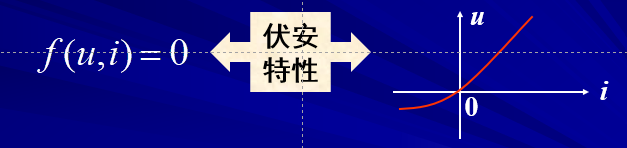
\includegraphics[width=0.7\linewidth]{screenshot111}
	\caption{电阻的伏安特性曲线}
	\label{fig:screenshot111}
\end{figure}
\begin{equation}
	i=\frac{u}{R}=Gu
\end{equation}
其中G为电导,单位为S。

\noindent \textbf{注意:}
\begin{enumerate}
	\item 欧姆定律只适用于线性电阻($R$为常数)
	\item 如电阻上的电压与电流参考方向\textbf{非关联,公式中应冠以负号}	
	\item 说明线性电阻是无记忆、双向性的元件。
\end{enumerate}
功率:电阻元件在任何时刻总是消耗功率的。
\begin{figure}[H]
	\centering
	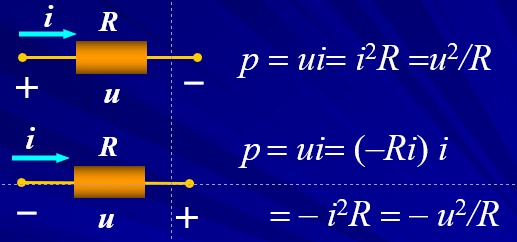
\includegraphics[width=0.7\linewidth]{screenshot112}
	\caption{电阻消耗功率图}
	\label{fig:screenshot112}
\end{figure}

能量:从$t_0$到$t$电阻消耗(吸收)的电能:
\begin{equation}
	W_R=\int_{t_0}^{t}pdt=\int_{t_0}^{t}uidt
\end{equation}

电阻的开路与短路:
\begin{figure}[H]
	\centering
	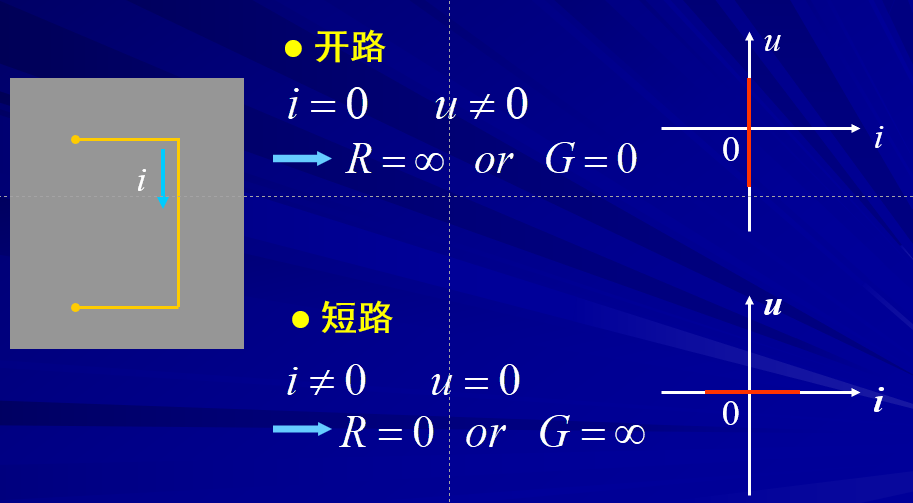
\includegraphics[width=0.7\linewidth]{screenshot113}
	\caption{电阻的开路与短路}
	\label{fig:screenshot113}
\end{figure}
\section{电压源和电流源}
\subsection{理想电压源}
定义:其两端电压总能保持定值或一定的时间函数,其值与流过它的电流$i$无关的元件叫理想电压源。
\begin{figure}[H]
	\centering
	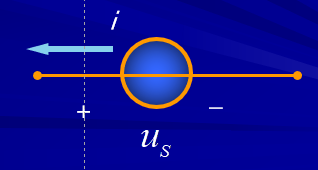
\includegraphics[width=0.3\linewidth]{screenshot114}
	\caption{理想电压源电路符号}
	\label{fig:screenshot114}
\end{figure}
\begin{figure}[H]
	\centering
	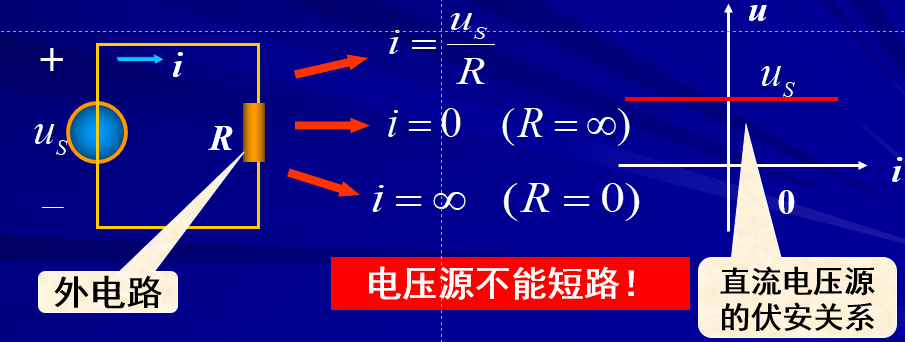
\includegraphics[width=0.6\linewidth]{screenshot115}
	\caption{理想电压源的电流电压关系}
	\label{fig:screenshot115}
\end{figure}
电压源的功率:$P=u_si]$
\begin{figure}
	\centering
	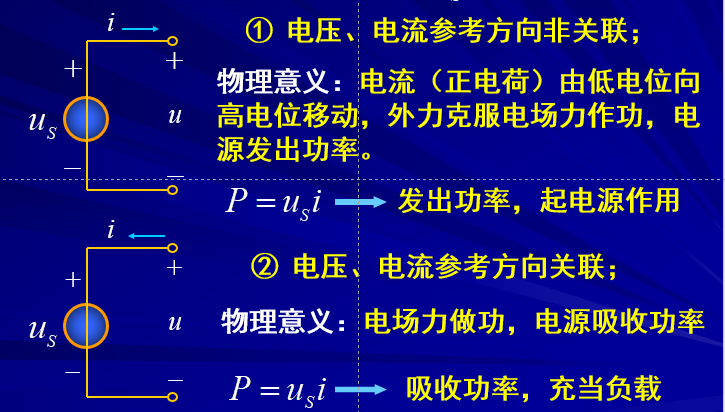
\includegraphics[width=0.6\linewidth]{screenshot116}
	\caption{电压源的功率}
	\label{fig:screenshot116}
\end{figure}
\subsection{理想电流源}
定义:其输出电流总能保持定值或一定的时间函数,其值与它的两端电压$u$无关的元件叫理想电流源。
\begin{figure}[H]
	\centering
	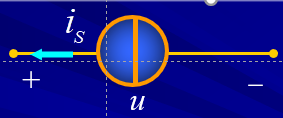
\includegraphics[width=0.3\linewidth]{screenshot117}
	\caption{理想电流源的电路符号}
	\label{fig:screenshot117}
\end{figure}
\begin{figure}[H]
	\centering
	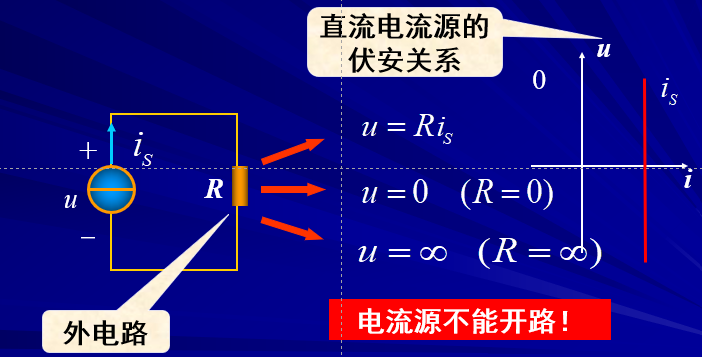
\includegraphics[width=0.6\linewidth]{screenshot118}
	\caption{理想电流源的电压电流关系}
	\label{fig:screenshot118}
\end{figure}
电流源的功率:$P=ui_s$
\begin{figure}[H]
	\centering
	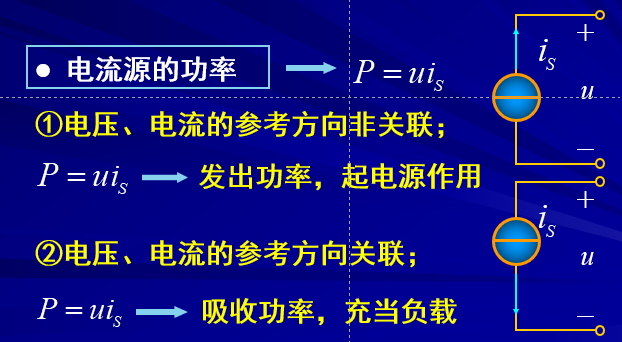
\includegraphics[width=0.6\linewidth]{screenshot119}
	\caption{电流源的功率}
	\label{fig:screenshot119}
\end{figure}
\subsection{受控电源(非独立源)}
定义:电压或电流的大小和方向不是给定的时间函数,而是受电路中某个地方的电压(或电流)控制的电源,称受控源。
\begin{figure}[H]
	\centering
	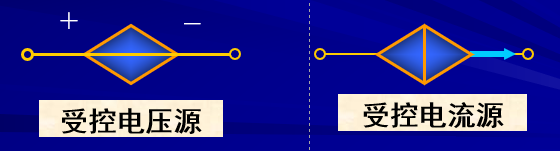
\includegraphics[width=0.4\linewidth]{screenshot120}
	\caption{受控电源的电路符号}
	\label{fig:screenshot120}
\end{figure}
受控源可分为四种类型:
\begin{enumerate}
	\item 电流控制的电流源(CCCS)
	
	\begin{figure}[h]
		\centering
		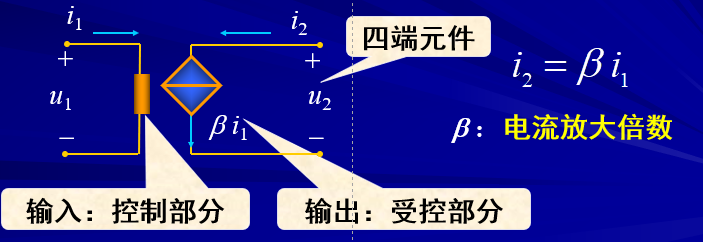
\includegraphics[width=0.5\linewidth]{screenshot121}
		\caption{CCCS}
		\label{fig:screenshot121}
	\end{figure}
	\item 电压控制的电流源(VCCS)
	\begin{figure}[H]
		\centering
		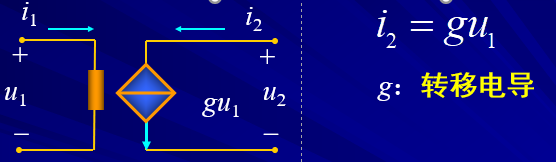
\includegraphics[width=0.5\linewidth]{screenshot122}
		\caption{VCCS}
		\label{fig:screenshot122}
	\end{figure}
	\item 电压控制的电压源(VCVS)\begin{figure}[H]
		\centering
		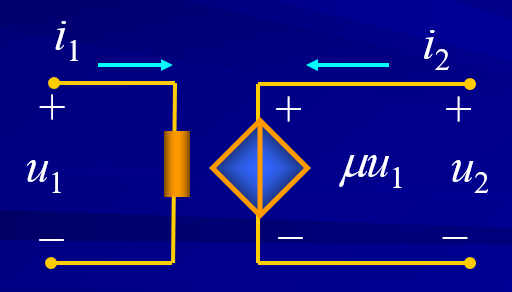
\includegraphics[width=0.5\linewidth]{screenshot123}
		\caption{VCVS}
		\label{fig:screenshot123}
	\end{figure}
	\item 电流控制的电压源(CCVS)
	\begin{figure}[H]
		\centering
		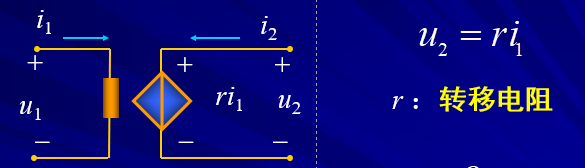
\includegraphics[width=0.5\linewidth]{screenshot124}
		\caption{CCVS}
		\label{fig:screenshot124}
	\end{figure}
\end{enumerate}
例题:\begin{figure}[H]
	\centering
	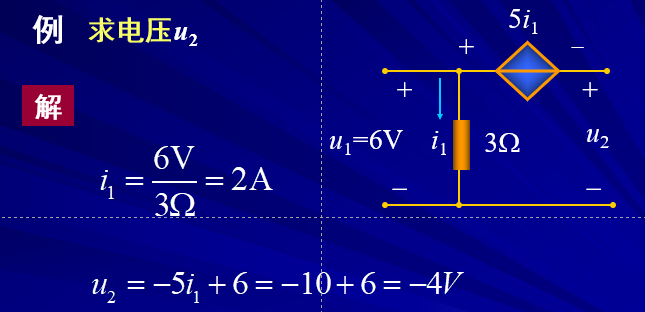
\includegraphics[width=0.7\linewidth]{screenshot125}
	\caption{受控电源例题}
	\label{fig:screenshot125}
\end{figure}

\section{基尔霍夫定律}
支路:电路中每一个两端元件就叫一条支路。电路中通过同一电流的分支。 \par 结点:元件的连接点称为结点。或三条以上支路的连接点称为结点。 \par 路径:两结点间的一条通路,由支路构成。\par 回路:由支路组成的闭合路径。 \par 对平面电路,其内部不含任何支路的回路称网孔。
\subsection{基尔霍夫电流定律(KCL)}
在集总参数电路中,任意时刻,对任意结点流出(或流入)该结点电流的代数和等于零。\textbf{流出取正,流入取负。}
\begin{equation}
	\sum_{b=1}^{m} i(t)=0 \quad or \quad \sum i_{\mbox{\scriptsize 入}}=\sum i_{\mbox{\scriptsize 出}}
\end{equation}
\textbf{KCL可推广应用于电路中包围多个结点的任一闭合面。}
\begin{figure}[H]
	\centering
	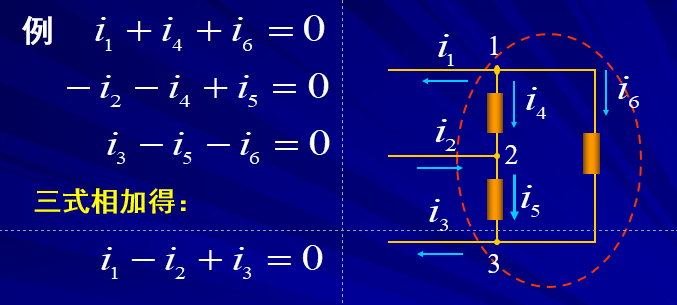
\includegraphics[width=0.4\linewidth]{screenshot126}
	\caption{KCL推广}
	\label{fig:screenshot126}
\end{figure}
\noindent\textbf{明确:}
\begin{enumerate}
	\item KCL是电荷守恒和电流连续性原理在电路中任意结点处的反映;
	\item KCL是对结点处支路电流加的约束,与支路上接的是什么元件无关,与电路是线性还是非线性无关;
	\item KCL方程是按电流参考方向列写的,与电流实际方向无关。
\end{enumerate}
\subsection{基尔霍夫电压定律(KVL)}
在集总参数电路中,任一时刻,沿任一回路,所有支路电压的代数和恒等于零。
\begin{equation}
	\sum_{b=1}^{m} u(t)=0 \quad or \quad \sum u_{\mbox{\scriptsize 降}}=\sum u_{\mbox{\scriptsize 升}}
\end{equation}
\textbf{KVL也适用于电路中任一假想的回路。}
\begin{figure}[H]
	\centering
	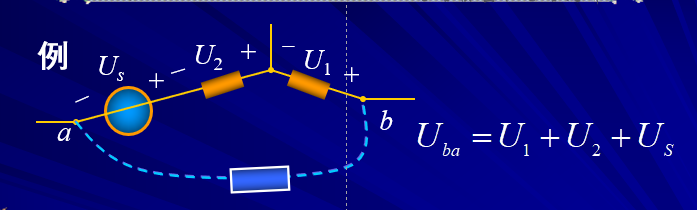
\includegraphics[width=0.5\linewidth]{screenshot127}
	\caption{KVL推广}
	\label{fig:screenshot127}
\end{figure}
\noindent\textbf{明确:}
\begin{enumerate}
	\item KVL的实质反映了电路遵从能量守恒定律;
	\item KVL是对回路中的支路电压加的约束,与回路各支路上接的是什么元件无关,与电路是线性还是非线性无关;
	\item KVL方程是按电压参考方向列写,与电压实际方向无关。
\end{enumerate}
\subsection{小结}
\begin{enumerate}
	\item KCL是对支路电流的线性约束,KVL是对回路电压的线性约束。
	\item KCL、KVL与组成支路的元件性质及参数无关。
	\item KCL表明在每一节点上电荷是守恒的;KVL是能量守恒的具体体现(电压与路径无关)。
	\item  KCL、KVL只适用于集总参数的电路。
\end{enumerate}
\section{思考与练习}
\begin{figure}[H]
	\centering
	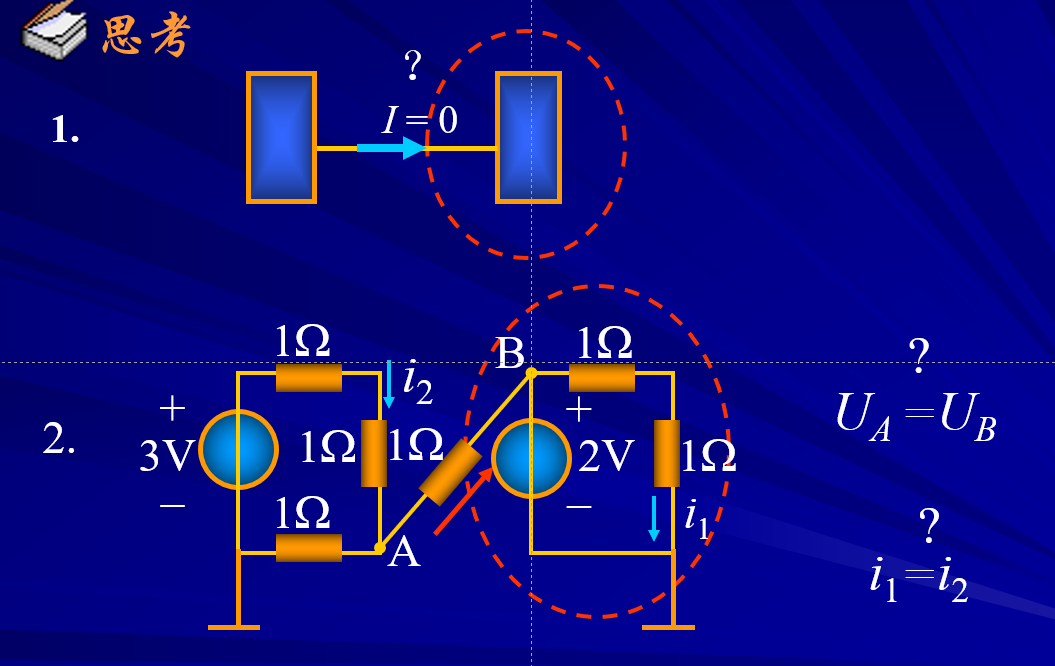
\includegraphics[width=0.7\linewidth]{screenshot128}
	\caption{思考题}
	\label{fig:screenshot128}
\end{figure}
\begin{enumerate}
	\item[1.] 由于电路未构成闭合回路,左端回路向右端回路输送电流,而右端并无返回电流,这不满足守恒定律,故I=0;
	\item[2.] 两独立回路分别接地,电路分析如下图所示:
	\begin{figure}[H]
		\centering
		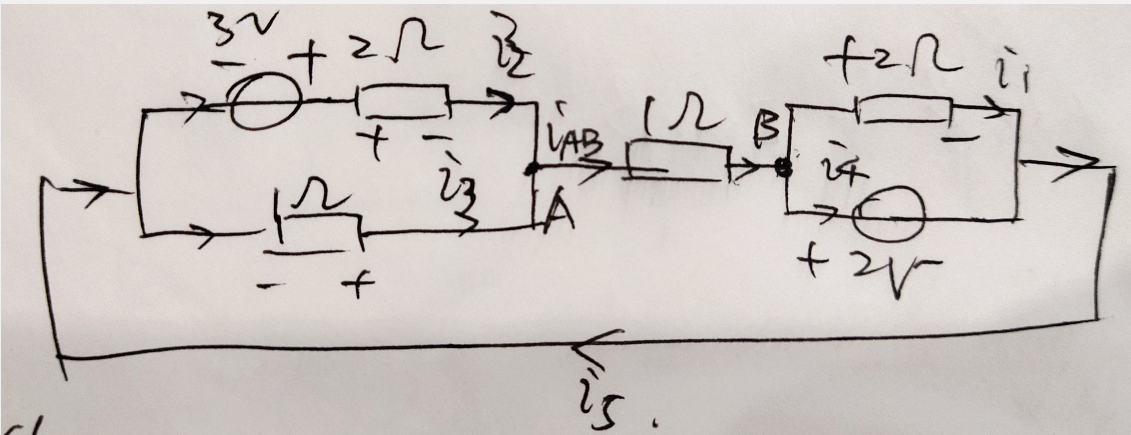
\includegraphics[width=0.5\linewidth]{screenshot013}
		\caption{}
		\label{fig:screenshot013}
	\end{figure}
	由KCL得:
	\begin{equation}
		\begin{aligned}
			i_2+i_3&=i_{AB} \\
			i_1+i_4&=i_{AB} \\
			i_2+i_3&=i_5 \\
			i_1+i_4&=i_5 \\
		\end{aligned}
	\end{equation}
	由KVL得:
	\begin{equation}
		\begin{aligned}
			-3V+2i_2-i_3&=0 \\
			2i_1-2A&=0 \\
		\end{aligned}
	\end{equation}
故$i_1=1A$,$i_{AB}=i_5$,由于电路构成闭合回路,所以$i_5$必不为零,所以$i_{AB} \neq 0$,所以A、B两点之间存在电势差,故$U_A \neq U_B$ ;  
由于两独立回路中电流均是从$i_5$中分流而来,而显然分流时$i_1 >i_2$,故$i_1 \neq i_2$
\end{enumerate}
~\\
~\\
课后习题:
~\\
1-10\qquad(1)求$i_1,u_{ab}$,(2)求$u_{cb}$ \quad 2.222A \quad  -13V
\begin{figure}[H]
	\centering
	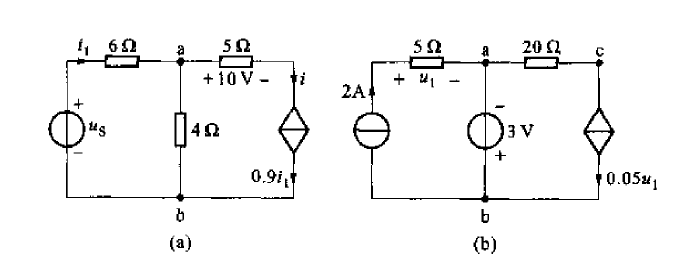
\includegraphics[width=0.7\linewidth]{screenshot011}
	\caption{题1-10图}
	\label{fig:screenshot011}
\end{figure}

\noindent1-12\qquad (1)$R_1,R_2,R_3不定$(2)$R_1=R_2=R_3$ (克拉姆法则)\par 在以上两种情况下,确定尽可能多的未知电流
\begin{figure}[H]
	\centering
	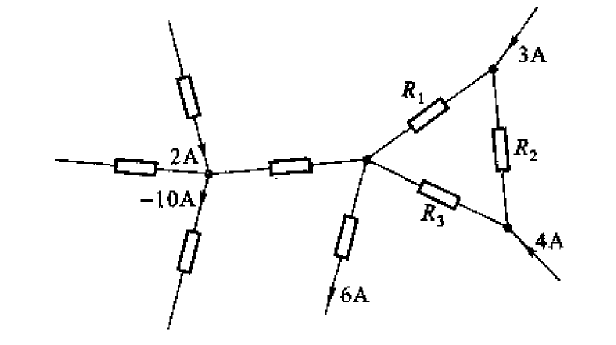
\includegraphics[width=0.5\linewidth]{screenshot012}
	\caption{}
	\label{fig:screenshot012}
\end{figure}

\chapter{电阻电路的等效变换}
\section{引言}
不变线性电路(线性电路):由时不变线性无源元件、线性受控源和独立电源组成的电路 \par 线性电阻性电路(电阻电路):构成电路的无源元件均为线性电阻 \par
两端电路(网络):任何一个复杂的电路,向外引出两个端钮,且从一个端子流入的电流等于从另一端子流出的电流,则称这一电路为二端网络(或一端口网络)。
\section{电路的等效变换}
\begin{figure}[H]
	\centering
	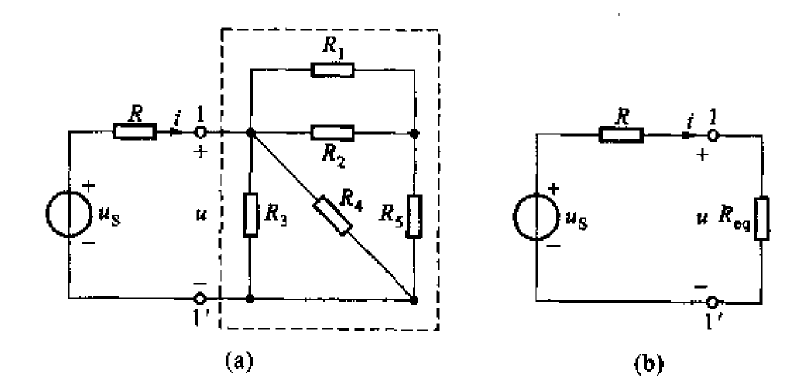
\includegraphics[width=0.4\linewidth]{screenshot129}
	\caption{等效电阻}
	\label{fig:screenshot129}
\end{figure}
当电路中某一部分用其等效电路代替后,未被代替部分的电压和电流均应保持不变。也就是说,用等效电路的方法求解电路时,电压和电流保持不变的部分仅限于等效电路以外,这就是“对外等效”的概念。等效电路是被代替部分的简化或结构变形,因此,内部并不等效。
\section{电阻的串联和并联}
\subsection{电阻的串联}
\begin{figure}[H]
	\centering
	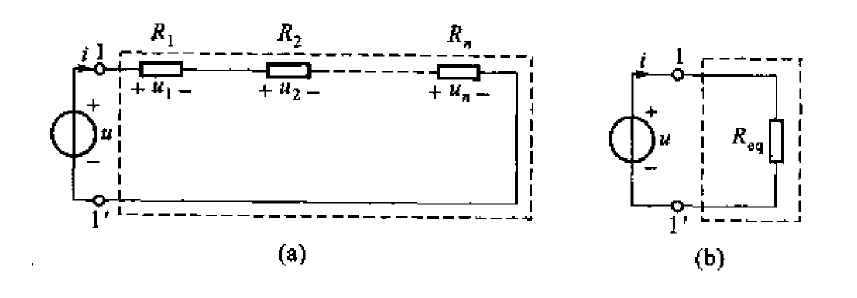
\includegraphics[width=0.5\linewidth]{screenshot130}
	\caption{串联}
	\label{fig:screenshot130}
\end{figure}
\begin{equation}
	R_{eq}=\sum_{k=1}^{n} R_k
\end{equation}
各电阻上的电压(分压公式)为:
\begin{equation}
	u_k=R_ki=\frac{R_k}{R_{eq}}u \quad k=1,2,...,n
\end{equation}
\subsection{电阻的并联}
\begin{figure}[H]
	\centering
	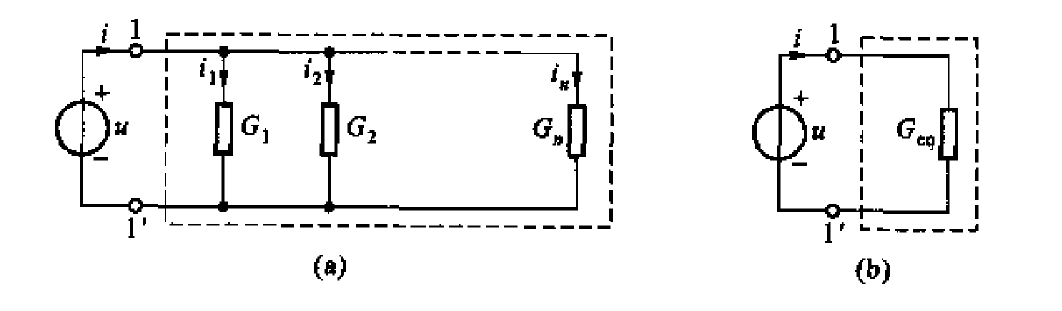
\includegraphics[width=0.5\linewidth]{screenshot131}
	\caption{并联}
	\label{fig:screenshot131}
\end{figure}
\begin{equation}
	\begin{aligned}	
		G_{eq}&=\sum_{k=1}^{n}G_k \\	
		R_{eq}&=\frac{1}{G_{eq}}=\frac{1}{\sum_{k=1}^{n} 1/R_k} \\
		\frac{1}{R_{eq}}&=\sum_{k=1}^{n}\frac{1}{R_k} \\
	\end{aligned}
\end{equation}
各电阻中的电流(分流公式)为:
\begin{equation}
	i_k=G_ku=\frac{G_k}{G_{eq}}i \quad k=1,2,...,n
\end{equation}
当n=2时,等效电阻及各电阻的分流值为
\begin{equation}
	\begin{aligned}
		R_{eq}&=\frac{1}{1/R_1+1/R_2}=\frac{R_1R_2}{R_1+R_2} \\
		i_1&=\frac{G_1}{G_{eq}}i=\frac{R_2}{R_1+R_2}i \\
	\end{aligned}
\end{equation}
\subsection{其他连接方式}
混联、桥联
\begin{figure}[H]
	\centering
	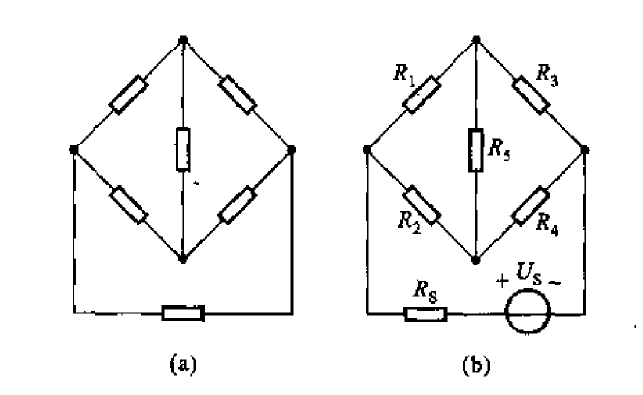
\includegraphics[width=0.4\linewidth]{screenshot132}
	\caption{桥形结构与惠斯通电桥}
	\label{fig:screenshot132}
\end{figure}
当满足$R_1R_4=R_2R_3$时,对角线之路中电流为0,处于电桥平衡状态,此时$R_5$可看作开路或短路。
\subsection{例题}
\noindent\textbf{例题2:}
\begin{figure}[H]
	\centering
	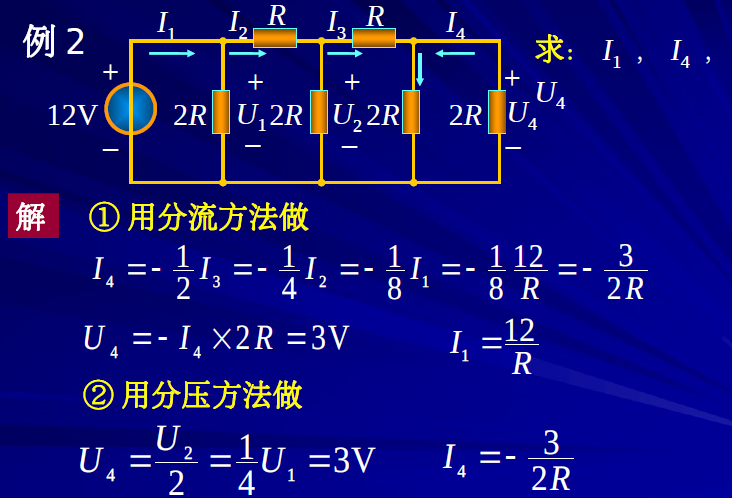
\includegraphics[width=0.5\linewidth]{screenshot001}
	\caption{例题2}
	\label{fig:screenshot001}
\end{figure}
从以上例题可得求解串、并联电路的一般步骤:
\begin{enumerate}
	\item 求出等效电阻或等效电导
	\item 应用欧姆定律求出总电压或总电流
	\item 应用欧姆定律或分压、分流公式求各电阻上的电
	流和电压
\end{enumerate}
\newpage
\noindent\textbf{例题4:}
求$R_{ab}$  \quad   res:$R_{ab}=70\Omega$   
\begin{figure}[H]
	\centering
	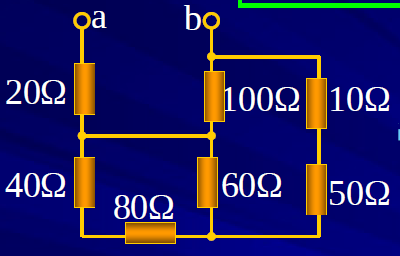
\includegraphics[width=0.4\linewidth]{screenshot002}
	\caption{例题4图}
	\label{fig:screenshot002}
\end{figure}
\noindent\textbf{例题5:}
求$R_{ab}$\quad $R_{ab}=10\Omega$
\begin{figure}[H]
	\centering
	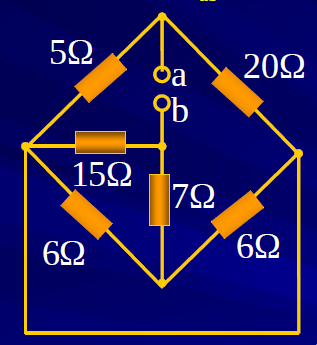
\includegraphics[width=0.3\linewidth]{screenshot003}
	\caption{例题5}
	\label{fig:screenshot003}
\end{figure}

\noindent\textbf{例题6:}
求$R_{ab}$\quad $R_{ab}=R$
\begin{figure}[H]
	\centering
	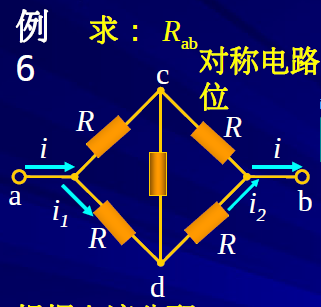
\includegraphics[width=0.3\linewidth]{screenshot004}
	\caption{例题6}
	\label{fig:screenshot004}
\end{figure}

\section{电阻的Y形联结和$\triangle$形联结的等效变换}
\subsection{电阻的$\triangle$和Y形连接}
\begin{figure}[H]
	\centering
	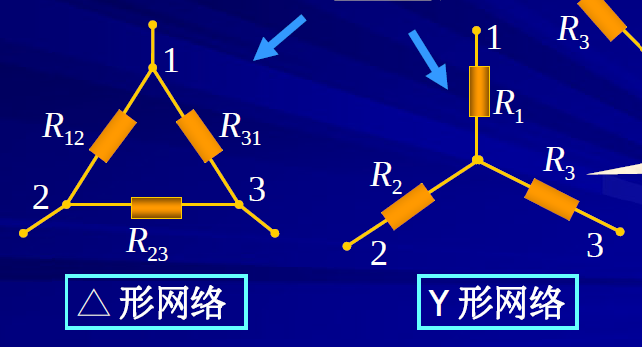
\includegraphics[width=0.5\linewidth]{screenshot005}
	\caption{两种连接方式示意图}
	\label{fig:screenshot005}
\end{figure}
$\triangle$和Y网络的变形:
\begin{figure}[H]
	\centering
	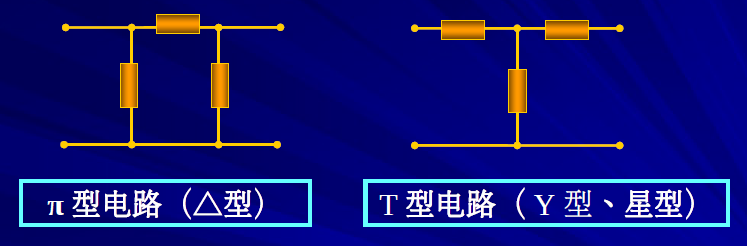
\includegraphics[width=0.5\linewidth]{screenshot006}
	\caption{连接方式的变形}
	\label{fig:screenshot006}
\end{figure}
\subsection{$\triangle$-Y变换的等效条件}
\noindent Y$\rightarrow$$\triangle$:
\begin{equation}
	\begin{aligned}
		R_{12}&=\frac{R_1R_2+R_2R_3+R_3R_1}{R_3} \\[6pt]
		R_{23}&=\frac{R_1R_2+R_2R_3+R_3R_1}{R_1} \\[6pt]
		R_{31}&=\frac{R_1R_2+R_2R_3+R_3R_1}{R_2} \\
	\end{aligned}
\end{equation}
等效于:
\begin{equation}
	\begin{aligned}
		R_{12}&=\frac{G_1G_2}{G_1+G_2+G_3} \\[6pt]
		R_{23}&=\frac{G_2G_3}{G_1+G_2+G_3} \\[6pt]
		R_{31}&=\frac{G_3G_1}{G_1+G_2+G_3} \\[6pt]
	\end{aligned}
\end{equation}
$\triangle$$\rightarrow$Y:
\begin{equation}
	\begin{aligned}
		R_1&=\frac{R_{12}R_{31}}{R_{12}+R_{23}+R_{31}} \\[6pt]
		R_2&=\frac{R_{23}R_{12}}{R_{12}+R_{23}+R_{31}} \\[6pt]
		R_3&=\frac{R_{23}R_{31}}{R_{12}+R_{23}+R_{31}} \\
	\end{aligned}
\end{equation}
简记为:
\begin{equation}
	\begin{aligned}
		R_Y&=\frac{\triangle\mbox{形相邻电阻的乘积}}{\triangle \mbox{形电阻之和}} \\
		R_\triangle&=\frac{\mbox{Y形电阻两两乘积之和}}{\mbox{Y形不相邻电阻}}
	\end{aligned}
\end{equation}
\noindent\textbf{特例:}
~\\
若三个电阻相等,则有:
$R_\triangle=3R_Y$
\begin{figure}[H]
	\centering
	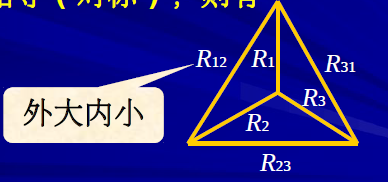
\includegraphics[width=0.4\linewidth]{screenshot007}
	\caption{}
	\label{fig:screenshot007}
\end{figure}

\subsection{例题}
\noindent\textbf{例题1:}
\begin{figure}[H]
	\centering
	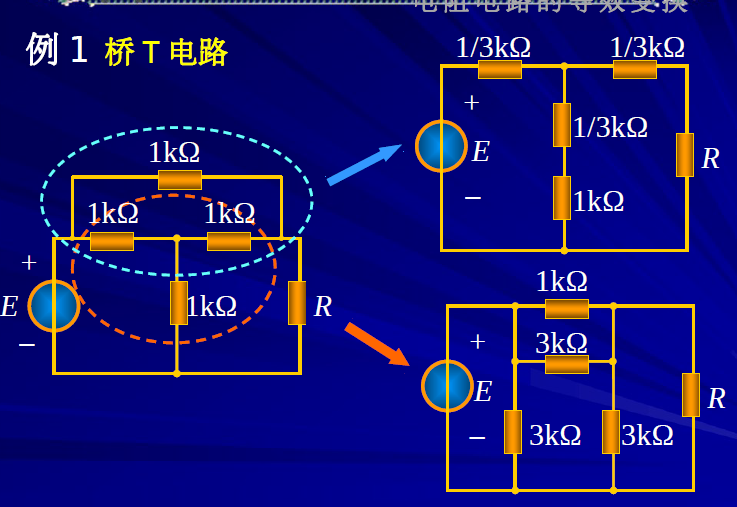
\includegraphics[width=0.7\linewidth]{screenshot008}
	\caption{桥T电路}
	\label{fig:screenshot008}
\end{figure}
\newpage
\noindent\textbf{例题2:}
计算90$\Omega$电阻的吸收功率 \quad P=3.6W
\begin{figure}[H]
	\centering
	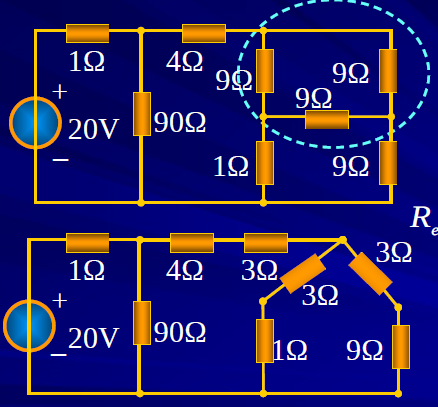
\includegraphics[width=0.5\linewidth]{screenshot009}
	\caption{}
	\label{fig:screenshot009}
\end{figure}
\noindent\textbf{例题3:}
求负载电阻$R_L$消耗的功率 \quad $P_L=40W$
\begin{figure}[H]
	\centering
	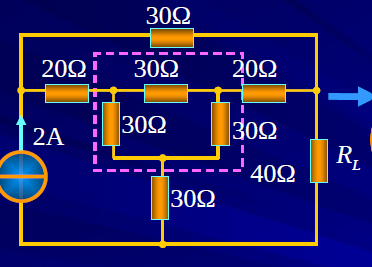
\includegraphics[width=0.5\linewidth]{screenshot010}
	\caption{}
	\label{fig:screenshot010}
\end{figure}
\newpage
\section{电压源、电流源的串并联}
n个电压源的串联可用一个电压源等效替代:
\begin{equation}
	u_S=u_{S1}+u_{S2}+...+u_{Sn}=\sum_{k=1}^{n} u_{Sk}
\end{equation}
若参考方向一致,则取+,否则取-。
\begin{figure}[H]
	\centering
	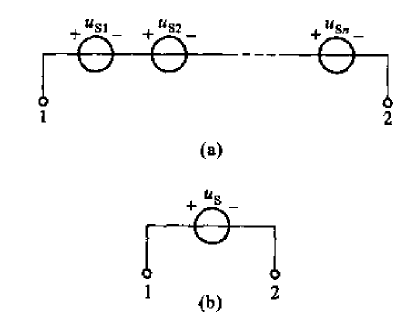
\includegraphics[width=0.4\linewidth]{screenshot014}
	\caption{电压源的串联}
	\label{fig:screenshot014}
\end{figure}
\noindent\textbf{强调:当!独立!(受控的不可以)电压源与任意元件并联时,都等效为一个单一的电压源!!!}
\begin{figure}[H]
	\centering
	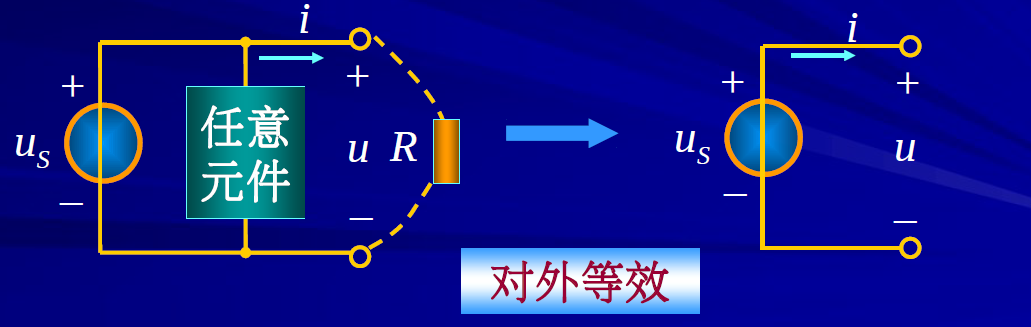
\includegraphics[width=0.5\linewidth]{screenshot021}
	\caption{电压源与支路的并联等效}
	\label{fig:screenshot021}
\end{figure}

n个电流源的并联可用一个电流源等效替代:
\begin{equation}
	i_S=i_{S1}+i_{S2}+...+i_{Sn}=\sum_{k=1}^{n} i_{Sk}
\end{equation}
若参考方向一致,则取+,否则取-。
\begin{figure}[H]
	\centering
	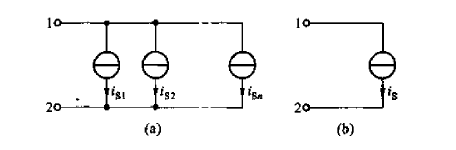
\includegraphics[width=0.5\linewidth]{screenshot015}
	\caption{电流源的并联}
	\label{fig:screenshot015}
\end{figure}
\noindent\textbf{强调:当!!独立!!(受控的不可以)电流源与任意元件串联时,都等效为一个单一的电流源!!!}
\begin{figure}[H]
	\centering
	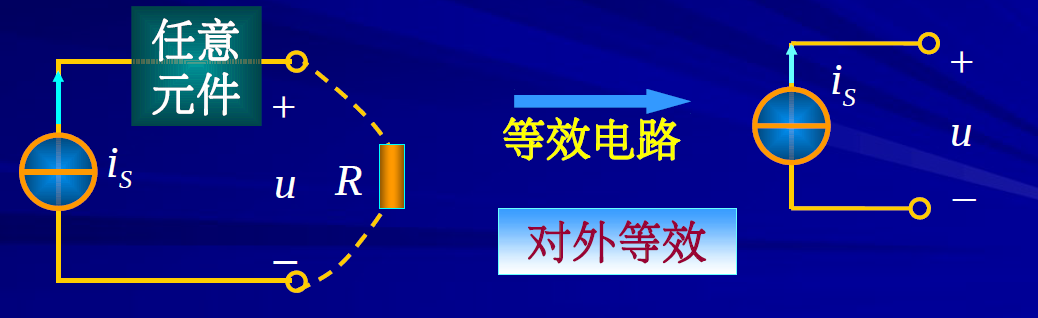
\includegraphics[width=0.5\linewidth]{screenshot022}
	\caption{电流源与支路的串联等效}
	\label{fig:screenshot022}
\end{figure}


只有激励电压相等且极性一致的电压源才允许并联,否则违背KVL。其等效电路为其中任一电压源,但是这个并联组合向外部提供的电流在各个电压源之间如何分配则无法确定。

只有激励电流相等且方向一致的电流源才允许串联,否则违背KCL。其等效电路为其中任一电流源,但是这个串联组合向的总电压在各个电流源之间如何分配则无法确定。
\section{实际电源的两种模型及其等效变换}
\begin{figure}[H]
	\centering
	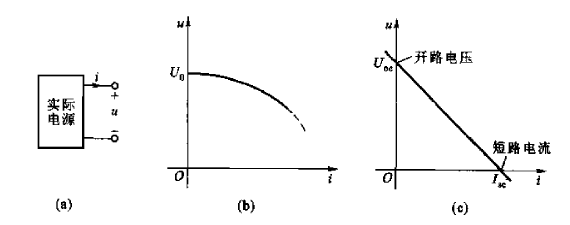
\includegraphics[width=0.7\linewidth]{screenshot016}
	\caption{实际电源及其伏安特性曲线}
	\label{fig:screenshot016}
\end{figure}
当$i=0$时,开路电压$U_{oc}$;当$u=0$时,短路电流$I_{sc}$。根据此伏安特性曲线,可以用\textbf{电压源和电阻的串联组合或电流源和电导的并联组合}作为实际电源的电路模型。
\begin{figure}[H]
	\centering
	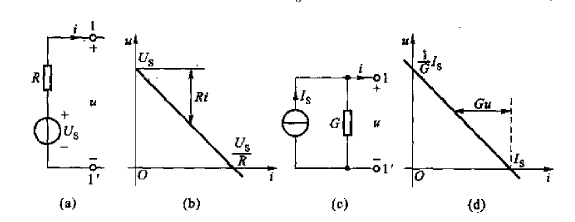
\includegraphics[width=0.7\linewidth]{screenshot017}
	\caption{电源的两种电路模型}
	\label{fig:screenshot017}
\end{figure}
\noindent 图2.17(a)所示为电压源$U_S$和电阻R的串联组合,端子处满足:
\begin{equation}
	u=U_S-Ri
\end{equation}
图2.17(b)所示为电压源$I_S$和电导G的并联组合,端子处满足:
\begin{equation}
	i=I_S-Gu
\end{equation}
若满足:
\begin{equation}
	G=\frac{1}{R},I_S=GU_S
\end{equation}
则(2.11)(2.12)则完全相同。(2.13)式即为这两种组合对外等效的必要条件。(\textbf{注意参考方向,$I_S$的参考方向由$U_S$的负极指向正极})

\noindent\textbf{注意:}这种等效变换仅保证端子外部电路的电压、电流和功率相同,对内部无等效可言。

受控电压源、电阻的串联组合,受控电流源、电导的并联组合也可以进行等效变换。

\noindent \textbf{例题1:}
求(a)中电流$i$。
\begin{figure}[H]
	\centering
	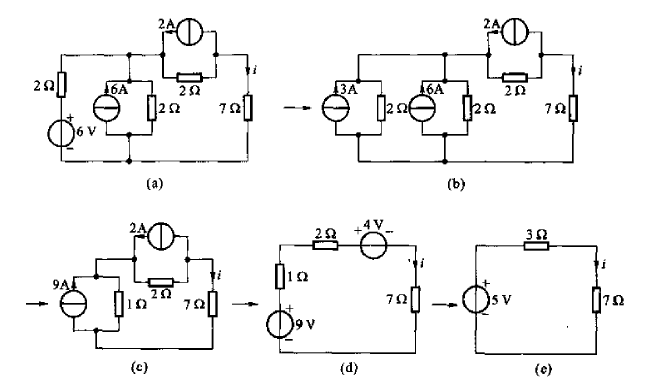
\includegraphics[width=0.5\linewidth]{screenshot018}
	\caption{例题1}
	\label{fig:screenshot018}
\end{figure}

\noindent \textbf{例题2:}
已知$u_S=12V,R=2\Omega,i_c$受电阻R上的电压$u_R$控制,且$i_c=gu_R,g=2S$。求$u_R$
\begin{figure}[H]
	\centering
	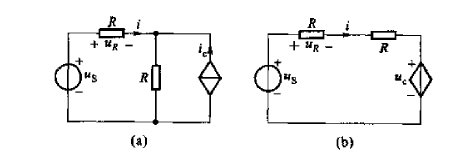
\includegraphics[width=0.5\linewidth]{screenshot019}
	\caption{例题2}
	\label{fig:screenshot019}
\end{figure}
课堂练习:
\begin{figure}[H]
	\centering
	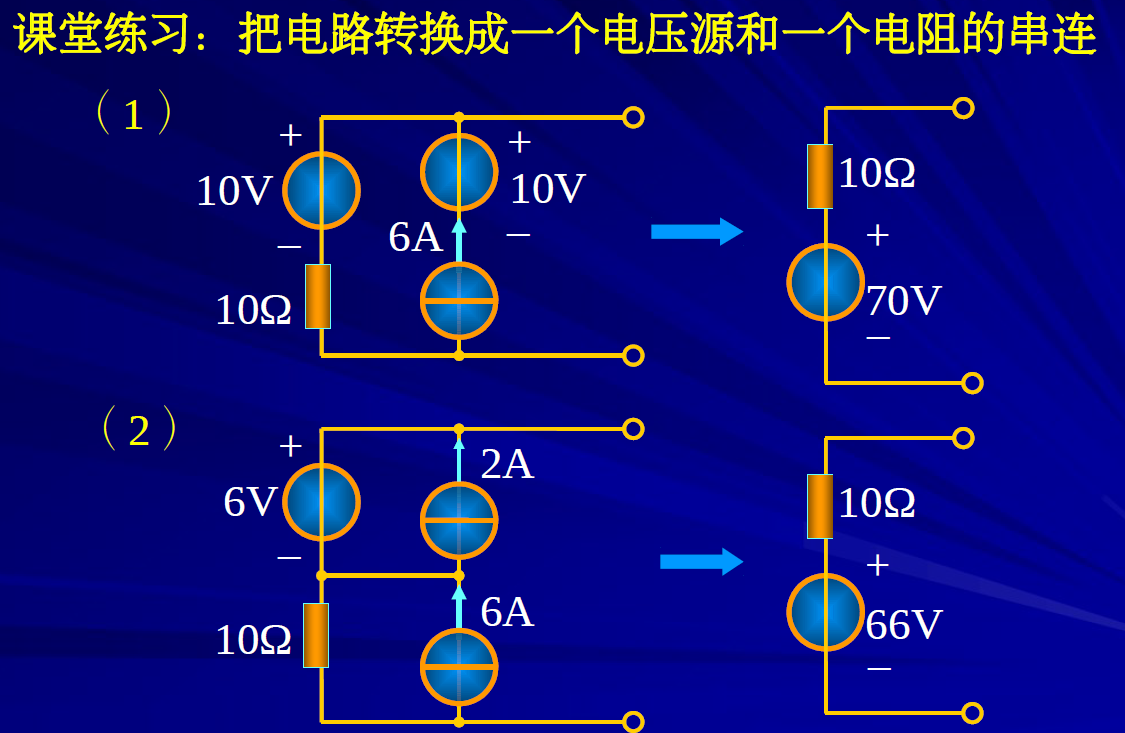
\includegraphics[width=0.5\linewidth]{screenshot023}
	\caption{课堂练习}
	\label{fig:screenshot023}
\end{figure}
\newpage
\noindent\textbf{例题3:}求电流$i$
\begin{figure}[H]
	\centering
	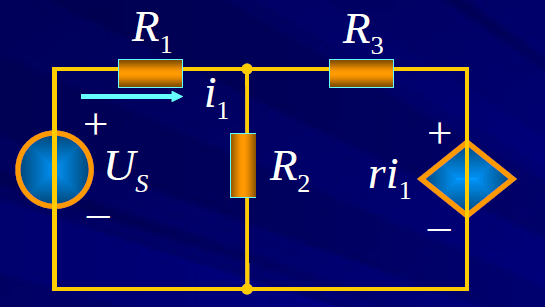
\includegraphics[width=0.5\linewidth]{screenshot024}
	\caption{}
	\label{fig:screenshot024}
\end{figure}
\noindent\textbf{例题4}:把电路转换成一个电压源和一个电阻的串联
\begin{figure}[H]
	\centering
	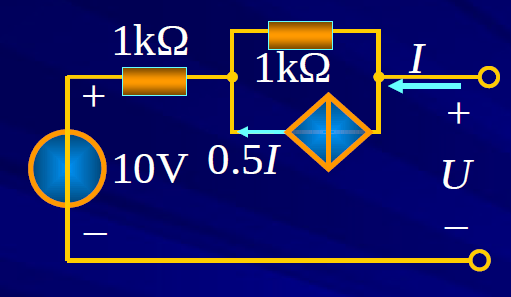
\includegraphics[width=0.5\linewidth]{screenshot025}
	\caption{}
	\label{fig:screenshot025}
\end{figure}
\textbf{注意:受控源在某些情况也可等效为电阻!}
\section{输入电阻}
定义一端口的输入电阻$R_i$为:
\begin{equation}
	R_i=\frac{u}{i}
\end{equation}
$u$为端口电压,$i$为端口电路i。端口的输入电阻即为端口的等效电阻。
求端口电阻的一般方法为电压、电流法。

\noindent\textbf{书例题1:}
求一端口的输入电阻
\begin{figure}[H]
	\centering
	\includegraphics[width=0.6\linewidth]{screenshot020}
	\caption{例题1}
	\label{fig:screenshot020}
\end{figure}

\noindent\textbf{例1:}
(1)
\begin{figure}[H]
	\centering
	\includegraphics[width=0.6\linewidth]{screenshot026}
	\caption{}
	\label{fig:screenshot026}
\end{figure}
先把有源网络的独立源置零:电压源短路;电流源开路,再求输入电阻。
$R_{in}=(R_1+R_2)//R_3$.

(2)
\begin{figure}[H]
	\centering
	\includegraphics[width=0.6\linewidth]{screenshot027}
	\caption{}
	\label{fig:screenshot027}
\end{figure}
外加电压源时将内电路所有独立源置零,再直接将$U,I$分别都用$i_1$表示出来,或者将受控电压源等效为一个4$\Omega$的等效电阻,则通过串并联即可解出结果$R_{in}=6\Omega$。
同理见第三题:

(3)
\begin{figure}[H]
	\centering
	\includegraphics[width=0.6\linewidth]{screenshot028}
	\caption{}
	\label{fig:screenshot028}
\end{figure}
可按题设方法逐步求解,也可以直接将受控电流源等效为一个10$\Omega$的电阻.则直接求出$R_{in}=11\Omega$
~\\

当存在受控源时,在一定的参数条件下,$R_i$有可能是0,也有可能是负值。负电阻元件实际是一个发出功率的元件。
\section{思考与练习}
课后习题(P47):

\noindent\textbf{2-4} 求等效电阻$R_{ab}$
\begin{figure}[H]
	\centering
	\includegraphics[width=0.7\linewidth]{screenshot030}
	\caption{2-4}
	\label{fig:screenshot030}
\end{figure}
参考答案见下页
\begin{enumerate}
	\item[(1)](d)中也可以直接对$R_2$利用Y-$\Delta$变换,再用串并联电路求解;
	\item[(2)](e)中是利用了等电势法将电路分为几部分再进行求解;
	\item[(3)](f)中也可以先对右侧的1$\Omega$,2$\Omega$,2$\Omega$三个元件进行Y形变换,然后再次利用该变换步步转化求解;
	\item[(4)](g)中同样利用了等电势法,将长方体分割为三部分并联求解。
\end{enumerate}
\noindent\textbf{2-3}:题目见书

注意区分$u_0$和$u_{ot}$以及电压表的内阻大小
\begin{figure}[H]
	\centering
	\includegraphics[width=0.3\linewidth]{screenshot029}
	\caption{2-3}
	\label{fig:screenshot029}
\end{figure}

\begin{figure}[H]
	\centering
	\includegraphics[width=0.7\linewidth]{2-4}
	\caption{2-4解答}
	\label{fig:2-4}
\end{figure}

\newpage
\noindent\textbf{2-8} 求对角线电压U及总电压$U_{ab}$ \quad 注意利用Y形变换后U仍然保持并没有消失
\begin{figure}[H]
	\centering
	\includegraphics[width=0.5\linewidth]{screenshot032}
	\caption{2-8}
	\label{fig:screenshot032}
\end{figure}

\noindent\textbf{2-9}
(2)题目见书,可对上部分进行Y形变换,也可以将下部分Y变为$\Delta$,此题第二种方法略显简单
\begin{figure}[H]
	\centering
	\includegraphics[width=0.4\linewidth]{screenshot033}
	\caption{2-9}
	\label{fig:screenshot033}
\end{figure}
\noindent\textbf{2-12}
求$\frac{u_0}{u_s}$,注意$u_0$在进行电源等效变换后所表示的是受控电流源和$R_4$一起两端的电压!
\begin{figure}[H]
	\centering
	\includegraphics[width=0.5\linewidth]{screenshot034}
	\caption{2-12}
	\label{fig:screenshot034}
\end{figure}
\newpage
\noindent\textbf{2-15(b)}
求输入电阻$R_i$,注意$u_1=u_{\mbox{\scriptsize 外加}}$。
\begin{figure}[H]
	\centering
	\includegraphics[width=0.5\linewidth]{screenshot035}
	\caption{2-15(b)}
	\label{fig:screenshot035}
\end{figure}

\noindent\textbf{2-16}
电路中全部电阻为1$\Omega$,求输入电阻$R_i$。

在电源等效变换时,尽可能地将电阻都转移到主电路上,通过多次的电压电流源转换,以减少并联支路,降低电路复杂性。同时注意:\textbf{受控电压电流源并联/串联任意电路时,不可如独立电压电流源一样忽略并联/串联支路}
\begin{figure}[H]
	\centering
	\includegraphics[width=0.5\linewidth]{screenshot036}
	\caption{2-16}
	\label{fig:screenshot036}
\end{figure}

\chapter{电阻电路的一般分析}
\section{电路的图}
在电路中通常指定每一条支路中的电流参考方向,电压一般取关联参考方向。
\section{KCL和KVL的独立方程数}
可以证明,对于具有n个结点的电路,\textbf{在任意(n-1)个结点上可以得出(n-1)个独立的KCL方程。}相应的(n-1)个结点称为独立结点。

当图G的任意两结点之间至少存在一条路径时,图G就称为连通图。

连通图G的树T定义为:包含图G的全部结点且不包含任何回路的连通子图。
树中包含的支路成为该树的树枝,而其他支路成为对应于该树的连支。

\textbf{任一个具有n个结点的连通图,它的任何一个树的树支数为(n-1)。}

单连支回路(基本回路):对于图G的任意一个树,加人一个连支后,就会形成一个回路,并且此回路除所加连支外均由树支组成。

由连支组成的全部基本回路构成基本回路组,基本回路的个数等于连支数。如果对基本回路组列写KVL方程,由于每个连支只在一个回路中出现,因此这些KVL方程必构成\textbf{独立方程组}。换言之,根据基本回路所列出的KVL方程组是独立方程。对一个具有b条支路和n个结点的电路连支数
\begin{equation}
	l=b-n+1
\end{equation}由于n个结点,则其数有n-1个支路,所以连支为b-(n-1),这也就是一个图的独立回路的数目。选择不同的树,就可以得到不同的基本回路组。

如果把一个图画在平面上,能使它的各条支路除连接的结点外不再交叉,这
样的图称为平面图,否则称为非平面图。平面图的全部网孔是一组独立回路,所以平面图的网孔数也就是独立回路数。

一个电路的KVL独立方程数等于它的独立回路数。如下图所示,取支路(1,4,5)为树,则三个基本回路为(1,3,5)、(1,2,4,5)、(4,5,6),则可以列出KVL方程如下
\begin{equation}
	\begin{aligned}
		&u_1+u_3+u_5=0 \\
		&u_1-u_2+u_4+u_5=0 \\
		&u_4+u_5-u_6=0 \\
	\end{aligned}
\end{equation}
\begin{figure}[H]
	\centering
	\includegraphics[width=0.7\linewidth]{screenshot031}
	\caption{基本回路的KVL方程}
	\label{fig:screenshot031}
\end{figure}

\section{支路电流法}
对一个具有b条支路和n个结点的电路,当以支路电压和支路电流为电路变量列写方程时,总计有2b个未知量\textbf{。根据KCL可以列出(n-1)个独立方程根据KVL可以列出(b-n+1)个独立方程;根据元件的VCR又可列出b个方程。}总计方程数为2b,与未知量数目相等。因此,可由2b个方程解出2b个
支路电压和支路电流。这种方法称为2b法。

为了减少求解的方程数,可以利用元件的VCR将各支路电压以支路电流
表示,然后代入KVL方程,这样,就得到以b个支路电流为未知量的b个KCL
和KVL方程。方程数从2b减少至b。这种方法称为支路电流法。

\begin{figure}[H]
	\centering
	\includegraphics[width=0.7\linewidth]{screenshot037}
	\caption{支路电流法}
	\label{fig:screenshot037}
\end{figure}

如上图所示,利用元件VCR的六个等式、选择网孔作为独立回路列出的3个KVL方程以及任意三个独立结点列出的KCL方程,组成支路电流法的全部方程:
\begin{equation}
	\left.
	\begin{aligned}
		&i_1=i_2+i_6 \\
		&i_2=i_4+i_3 \\
		&i_5=i_4+i_6 \\
		&i_1R_1+i_2R_2+i_3R_3=u_{S1} \\
		&i_4R_4+i_5R_5-i_3R_3=-R_5i_{S5} \\
		&i_6R_6-i_4R_4-i_2R_2=0 \\
	\end{aligned}
	\right\}
\end{equation}
式中的KVL方程可归纳为
\begin{equation}
	\sum i_kR_k=\sum u_{Sk}
\end{equation}
即在任一回路中,电阻电压的代数和等于电压源电压的代数和。

列出支路电流法的电路方程的步骤如下:
\begin{enumerate}\setlength{\itemsep}{0.2pt}
	\item[(1)]选定各支路电流的参考方向。
	\item[(2)]对$(n-1)$个独立结点列出KCL方程
	\item[(3)]选取$(b-n+1)$个独立回路,指定回路的绕行方向,按照式(3.4)列出KVL方程。
\end{enumerate}

\textbf{支路电流法要求b个支路电压均能以支路电流表示!!}

当电路中\textbf{含有理想电流源}时,避开理想电流源选取回路可以减少计算量!当电路中\textbf{含有受控源时},先将受控源看作独立源列方程;再将控制量用未知量表示,并代入所列方程,消去中间变量。

支路法列写的是KCL 和KVL 方程所以方程列写方便、直观,但方程数较多,宜于在支路数不多的情况下使用。
\section{网孔电流法}
在网孔电流法中,以网孔电流作为电路的独立变量,它仅适用于平画电路。
\begin{figure}[H]
	\centering
	\includegraphics[width=0.7\linewidth]{screenshot038}
	\caption{网孔电流法}
	\label{fig:screenshot038}
\end{figure}
将图中所有电流归结为由两个沿网孔连续流动的假想电流$i_{m1},i_{m2}$,则$i_1=i_{m1},i_3=i_{m2},i_2=i_{m1}-i_{m2}$。

由于网孔电流已经体现了电流连续即KCL的制约关系(换言之,根据网孔电流而计算的支路电流一定满足KCL方程,或称为自动满足KCL),所以用网孔电流作为电路变量求解时只需列出KVL方程。全部网孔是一组独立回路,因而对应的KVL方程将是独立的,且\textbf{独立方程个数与电路变量数均为全部网孔数},足以解出网孔电流。这种方法称为网孔电流法。

对图3.3可列出方程
\begin{equation}
	\left.
	\begin{aligned}
		R_2(i_{m1}-i_{m2})+u_{S2}-u_{S1}+i_{m1}R_1&=0 \\
		i_{m2}R_3+u_{S3}-u_{S2}-R_2(i_{m1}-i_{m2})&=0\\
	\end{aligned}
	\right\}
\end{equation}
用$R_{11},R_{22}$表示网孔1、2的自阻,即$R_{11}=R_1+R_2,R_{22}=R_2+R_3$,用$R_{12},R_{21}$表示两网孔的互阻,即共有电阻,即$R_{12}=R_{21}=-R_2$.

故(3.5)变为:
\begin{equation}
	\left.
	\begin{aligned}
		R_{11}i_{m1}+R_{12}i_{m2}&=u_{S1}-u_{S2} \\
		R_{21}i_{m1}+R_{22}i_{m2}&=u_{S2}-u_{S3} \\	\end{aligned}
	\right\}
\end{equation}
由于网孔绕行方向与网孔电流方向取为一致,故$R_{11},R_{22}$总为正值。当两网孔通过共有电阻上的网孔电流参考方向相同时,互阻取正,否则取负,若两网孔不相关,则取0。
\begin{figure}[H]
	\centering
	\includegraphics[width=0.7\linewidth]{screenshot039}
	\caption{网孔电流的一般形式}
	\label{fig:screenshot039}
\end{figure}
$u_{S11}...$为各网孔电压源电压的代数和。\textbf{方向与网孔电流一致时,取负号,否则取正号。}

当电路中存在电流源和电阻的并联组合时,可将它等效变换成电压源和电
阻的串联组合,再按上述方法进行分析。对于存在无伴电流源或受控源的情况,见下一章。

\section{回路电流法}
网孔电流法仅适用于平面电路,\textbf{回路电流法}则无此限制,它适用于平面或非平面电路。回路电流法是一种适用性较强并获得广泛应用的分析方法。

网孔电流是在网孔中连续流动的假想电流,对于一个具有b个支路,n个结点的电路,b个支路电流受(n-1)个KCL独立方程所制约,因此,\textbf{独立的支路电流只有(b-n+1)个}(b个未知数,n-1个方程,则基础解系中只有(b-n+1)个独立变量),等于网孔电流数。回路电流也是在回路中连续流动的假想电流。但是与网孔不同,回路的取法很多,选取的回路应是一组独立回路,且回路的个数(也即回略电流的个数)也应等于(b-n+1)个。选定一树以后形成的基本回路显然满足上述要求。这就是说,\textbf{基本回路电流}可以作为电路的独立变量来求解。

\textbf{例题:}已知$R_1,R_2,R_3,R_4,R_5,R_6,u_{S1},u_{S2}$,选择一组独立回路,列出回路电流方程。
\begin{figure}[H]
	\centering
	\includegraphics[width=0.6\linewidth]{screenshot040}
	\caption{回路电流}
	\label{fig:screenshot040}
\end{figure}
在三个基本回路列出以回路电流$I_{11},I_{22},I_{33}$为变量的KVL方程为:
\begin{equation}
	\left.
	\begin{aligned}
		&R_1I_{11}+u_{S1}+R_6(I_{11}-I_{13})+R_5(I_{11}+I_{12}-I_{13})-u_{S5}+R_4(I_{11}+I_{12})=0 \\
		&R_2I_{12}+R_5(I_{11}+I_{12}-I_{13})-u_{S5}+R_4(I_{11}+I_{12})=0 \\
		&R_6(I_{11}-I_{13})+R_3I_{13}+u_{S5}+R_5(I_{11}+I_{12}-I_{13})=0\\
	\end{aligned}
	\right\}
\end{equation}
对具有$l$个独立回路的电流可写出回路电流的一般形式:
\begin{figure}[H]
	\centering
	\includegraphics[width=0.6\linewidth]{screenshot042}
	\caption{}
	\label{fig:screenshot042}
\end{figure}
$R_{11},R_{22},R_{33}..$为各回路的自阻,$R_{12},R_{13}..$为回路间的互阻,$u_{S11},u_{S22}..$为各回路中所有电压源的代数和,\textbf{与电流方向一致时取负号}。

回路电流法的步骤可归纳如下:
\begin{enumerate}\setlength{\itemsep}{0.2pt}
	\item[(1)]根据给定的电路,通过选择一个树确定一组基本回路,并指定各回路电
	流参考方向。
	\item[(2)]按一般公式列出回路电流方程,注意自阻总是正的,互阻的正负由相关的两个回路电流通过共有电阻时两者的参考方向是否相同而定。并注意右边项取代数和时各有关电压源前面的正负号。
	\item[(3)]当电路中有受控源或无伴电流源时,需另行处理。
	\item[(4)]对于平面电路可用网孔电流法。
\end{enumerate}
若电路中有电流源和电阻的并联组合,则可等效变换为电压源和电阻。若电路中存在\textbf{无伴电流源},则将无伴电流源两端电压$U$作为一个 求解变量列入方程,再增加附加方程即可求解。或

当电路中含有受控电压源时,把它作为电压源暂时列于KVL方程的右边,同时把控制量用回路电流表示然后将用回路电流表示的受控源电压项移到方程的左边。当受控源是受控电流源时,可参照前面处理独立电流源的方法进行。或者有时可直接将方程简化,略过无伴电流源的电压,从而减少未知量。

\textbf{取回路时尽量使无伴电流源和无伴受控电流源都只有一个回路电流流过!}
\section{结点电压法}
在电路中任意选择某一结点为参考结点,其他结点为独立结点,这些结点与此参考结点之间的电压称为结点电压,结点电压的参考极性是以参考结点为负其余独立结点为正。由于任一支路都连接在两个结点上,根据KVL,支路电压就是两个结点电压之差。如果每一个支路电流都可由支路电压来表示,那么它一定也可以用结点电压来表示。在具有n个结点的电路中写出其中(n-1)个独立结点的KCL方程就得到变量为(n-1)个结点电压的共(n-1)个独立方程,称为结点电压方程,最后由这些方程解出结点电压,从而求出所需的电压、电流。这就是\textbf{结点电压法}。
\begin{equation}
	\sum i_{R_{out}}=\sum i_{S_{in}}
\end{equation}
即电阻流出电流之和等于电源流入电流之和。
\begin{figure}[H]
	\centering
	\includegraphics[width=0.7\linewidth]{screenshot043}
	\caption{结点电压法}
	\label{fig:screenshot043}
\end{figure}
如上图,结点1,2,3的KCL方程为
\begin{equation}
	\left.
	\begin{aligned}
		i_1+i_4+i_6&=0 \\
		i_2-i_4+i_5&=0 \\
		i_3-i_5-i_6&=0 \\
	\end{aligned}
\right\}
\end{equation}
由VCR等关系得:
\begin{figure}[H]
	\centering
	\includegraphics[width=0.6\linewidth]{screenshot044}
	\caption{}
	\label{fig:screenshot044}
\end{figure}
整理得:
\begin{figure}[H]
	\centering
	\includegraphics[width=0.6\linewidth]{screenshot045}
	\caption{}
	\label{fig:screenshot045}
\end{figure}
由此推出具有(n-1)个独立结点的电路,有:
\begin{figure}[H]
	\centering
	\includegraphics[width=0.8\linewidth]{screenshot046}
	\caption{}
	\label{fig:screenshot046}
\end{figure}
其中,$G_{11},G_{22}...$为结点的自导,等于结点引出的各支路电导之和,总为正;$G_{12},G_{21}...$为结点间的互导,互导总为负;方程右侧为结点的注入电流,流入取正,流出取负(注入电流源包括电压源和电阻串联组合经等效变换形成的电流源)

当电路中存在无伴电压源时,一种方法是将无伴电压源的电流作为附加变量列入KCL方程;另一种方法是将连接无伴电压源的两个结点电压方程合并为一个(若无伴电压源的一端是参考结点,则该结点的KCL方程解不列,仅补充以约束方程),\textbf{即取一个包含这两个结点的封闭面KCL,避免附加电流变量的出现},同时添加结点电压与无伴电压源的约束关系。

若电路中存在受控电流源,在建立结点电压方程时,先把控制量用结点电压表示,并暂时把它当作独立电流源,按上述方法列出结点电压方程然后把用结点电压表示的受控电流源电流项移到方程的左边。当电路中存在有伴受控电压源时,把控制量用有关结点电压表示并变换为等效受控电流源。如果存在无伴受控电压源,可参照无伴独立电压源的处理方法。

结点电压法的步骤可以归纳如下
\begin{enumerate}\setlength{\itemsep}{0.2pt}
	\item[(1)] 指定参考结点,其余结点对参考结点之间的电压就是结点电压。通常以参考结点为各结点电压的负极性。
	\item[(2)] 按一般公式列出结点电压方程,注意自导总是正的,互导总是负的;并注意各结点注入电流前面的“+”,“-”号。
	\item[(3)] 当电路中有受控源或无伴电压源时需另行处理。
\end{enumerate}
\textbf{选择参考节点时,尽量使无伴电压源的支路方程好列写,减少增加额外支路电流变量!}

\newpage
\noindent\textbf{例题:}列写结点电压法方程
\begin{figure}[H]
	\centering
	\includegraphics[width=0.5\linewidth]{screenshot049}
	\caption{例题图}
	\label{fig:screenshot049}
\end{figure}
注意参考结点的选择,使得$U_{n3}$支路无需再设置额外电流变量;此外注意\textbf{与电流源串接的电阻不参与列方程!}

\noindent\textbf{例题2:}求电压$U$和电流$I$ \quad  $U=195V,I=-120A$
\begin{figure}[H]
	\centering
	\includegraphics[width=0.5\linewidth]{screenshot050}
	\caption{}
	\label{fig:screenshot050}
\end{figure}
参考结点可选择上方或右侧结点均可。该题注意与电流源串联的电阻虽不参与计算,但由于对内不等效,\textbf{故仍需考虑其上的分压}!(该题也可运用回路法)
\section{思考与练习}
列出图示电路的结点电压方程。如果$R_s=0$,则方程又如何?(提示:为避免引人过多附加电流变量,对连有无伴电压源的结点部分,可在包含无伴电压源的封闭面S上写出KCL方程。)
\begin{figure}[H]
	\centering
	\includegraphics[width=0.7\linewidth]{screenshot077}
	\caption{}
	\label{fig:screenshot077}
\end{figure}




\chapter{电路定理}
\section{叠加定理}
\textbf{叠加定理}可表述为在线性电阻电路中,某处电压或电流都是电路中各个独立电源单独作用时,在该处分别产生的电压或电流的叠加。

使用登加定理时应注意以下几点
\begin{enumerate}\setlength{\itemsep}{0.2pt}
	\item[(1)] 叠加定理\textbf{只适用于线性电路},不适用于非线性电路。
	\item[(2)] 在叠加的各分电路中,不作用的电压源置零,在电压源处用短路代替;不作用的电流源置零,在电流源处用开路代替。电路中所有电阻都不予更动,\textbf{受控源则保留在各分电路中}。
	\item[(3)] 叠加时各分电路中的电压和电流的参考方向可以取为与原电路中的相同。取代数和时,应注意各分量前的“+”、“-”号。
	\item[(4)] \textbf{原电路的功率不等于按各分电路计算所得功率的叠加},这是因为功率是电压和电流的乘积,与激励不成线性关系。
\end{enumerate}

\noindent\textbf{例题1:}
\begin{figure}[H]
	\centering
	\includegraphics[width=0.7\linewidth]{screenshot047}
	\caption{例题1图}
	\label{fig:screenshot047}
\end{figure}
利用VCR等方法求出$U_1',U_1'',I_2',I_2''$,则原电路的总相应为
\begin{equation}
	\begin{aligned}
		U_1&=U_1'+U_1'' \\
		I_2&=I_2'+I_2'' \\
	\end{aligned}
\end{equation}

\noindent\textbf{例题2:}计算电压$u$,画出分电路图  \quad $u=17V$
\begin{figure}[H]
	\centering
	\includegraphics[width=0.5\linewidth]{screenshot051}
	\caption{例题2图}
	\label{fig:screenshot051}
\end{figure}
作出分电路图如下(叠加方式是任意的,可以一次一个独立源单独作用\textbf{,也可以一次几个独立源同时作用},取决于使分析计算简便).
\begin{figure}[H]
	\centering
	\includegraphics[width=0.7\linewidth]{screenshot052}
	\caption{分电路图}
	\label{fig:screenshot052}
\end{figure}
\begin{equation}
	\begin{aligned}
		&u^{(1)}=(6//3+1)\times 3=9V \\
		&9i_2-6V-12V=0 \\
		&u^{(2)}=6i_2-6+2=8V \\
	\end{aligned}
\end{equation}
其中第三个式子将右侧电路的电流源等效为电压源即可方便理解。故$u=17V$

\noindent\textbf{例题3:}
\begin{figure}[H]
	\centering
	\includegraphics[width=0.6\linewidth]{screenshot053}
	\caption{}
	\label{fig:screenshot053}
\end{figure}


在线性电路中,当所有激励(电压源和电流源)都同时增大或缩小K倍(K为实常数)时,响应(电压和电流〕也将同样增大或缩小K倍。这就是线性电路的\textbf{齐性定理},它不难从叠加定理推得。应注意,这里的激励是指\textbf{独立电源},并且\textbf{必须全部激励同时增大或缩小K倍},否则将导致错误的结果。显然,当电路中只有一个激励时,响应必与该激励成正比。

利用齐性定理分析梯形电路特别有效。

\noindent\textbf{例题4:}
求图中所示梯形电路各支路电流。
\begin{figure}[H]
	\centering
	\includegraphics[width=0.7\linewidth]{screenshot048}
	\caption{例题2图}
	\label{fig:screenshot048}
\end{figure}
本例计算是先从梯形电路最远离电源的一端开始,倒退至激励处。这种计算方法称为“倒退法”。先对某个电压或电流设一便于计算的值如本例设$i_5'=1A$,顺各支路推出$u_S'$的值,最后再按齐性定理予以修正。

\noindent\textbf{例题5:}求电流$i$。
\begin{figure}[H]
	\centering
	\includegraphics[width=0.7\linewidth]{screenshot054}
	\caption{}
	\label{fig:screenshot054}
\end{figure}

\section{替代定理}
替代定理的内容可叙述如下:在电路中如已求得$N_A$与$N_B$两个一端口网络连接端口的电压$u_p$与电流$i_p$,那么就可用一个$u_s=u_p$的电压源或一个$i_s=i_p$的电流源或用$R=u_p/i_p$的电阻来替代其中的一个网络,而使另一个网络的内部电压、电流均维持不变。替代后电路中全部电压和电流均保持原有值(解答唯一)
\begin{figure}[H]
	\centering
	\includegraphics[width=0.7\linewidth]{screenshot055}
	\caption{替代定理}
	\label{fig:screenshot055}
\end{figure}

\noindent\textbf{注意:}
\begin{enumerate}
	\item[1] 替代定理既适用于线性电路,也适用于非线性电路
	\item[2] 替代后电路必须有唯一解。\textbf{无电压源回路;无电流源结点(含广义结点)}
	\item[3] 替代后其余支路及参数不能改变
\end{enumerate}
\begin{figure}[H]
	\centering
	\includegraphics[width=0.5\linewidth]{screenshot056}
	\caption{替代后出现电压源回路的情形(必须避免)}
	\label{fig:screenshot056}
\end{figure}

\noindent\textbf{例题1:}若使$I_x=I/8$,求$R_x$  \quad $R_x=0.2\Omega$
\begin{figure}[H]
	\centering
	\includegraphics[width=0.5\linewidth]{screenshot057}
	\caption{例题1}
	\label{fig:screenshot057}
\end{figure}

如图所示进行替代后,再利用\textbf{叠加定理!!!}进行求解,左电路中注意电压的正负号以及与电阻上电压的关系($U_{BA}=\varphi_B-\varphi_A=U_{CA}-U_{DB}$),右电路中注意电压为负!
\begin{figure}[H]
	\centering
	\includegraphics[width=0.5\linewidth]{screenshot058}
	\caption{}
	\label{fig:screenshot058}
\end{figure}

\noindent\textbf{例题2:}求电流$I_1$ \quad $I_1=2.5A$
\begin{figure}[H]
	\centering
	\includegraphics[width=0.5\linewidth]{screenshot059}
	\caption{例题2}
	\label{fig:screenshot059}
\end{figure}
对电路简化后利用替代定理+叠加定理:
\begin{figure}[H]
	\centering
	\includegraphics[width=0.5\linewidth]{screenshot060}
	\caption{}
	\label{fig:screenshot060}
\end{figure}

\noindent\textbf{例题3:}已知$u_{ab}=0$,求电阻R(图中ab支路原先为一个1$\Omega$的电阻和一个3V的独立电压源)
\begin{figure}[H]
	\centering
	\includegraphics[width=0.3\linewidth]{screenshot061}
	\caption{例题3}
	\label{fig:screenshot061}
\end{figure}
利用替代定理和结点法,得R=6$\Omega$

\noindent\textbf{例题4:}
用多大电阻替代2V电压源而不影响电路的工作?
\begin{figure}[H]
	\centering
	\includegraphics[width=0.7\linewidth]{screenshot062}
	\caption{例题4}
	\label{fig:screenshot062}
\end{figure}
应求电流I,先化简电路,再应用叠加定理(注意电流流向正负号)(或结点法)得$R=2\Omega$

\noindent\textbf{例题5:}已知$u_{ab}=0$,求电阻R \quad R=15$\Omega$
\begin{figure}[H]
	\centering
	\includegraphics[width=0.5\linewidth]{screenshot063}
	\caption{例题5}
	\label{fig:screenshot063}
\end{figure}
可直接利用叠加定理将ac右端电路分离,则分析可变得更简单

\section{戴维宁定理和诺顿定理}
\subsection{戴维宁定理}
任何一个线性含源一端口网络,对外电路来
说,总可以用一个电压源和电阻的串联组合来等效置换;此电压源的电压等于外电路断开时端口处的开路电压$u_{oc}$,而电阻等于一端口的输入电阻(或等效电阻$R_{eq}$)。
\begin{figure}[H]
	\centering
	\includegraphics[width=0.5\linewidth]{screenshot064}
	\caption{戴维宁定理等效变换}
	\label{fig:screenshot064}
\end{figure}
定理的证明:
\begin{figure}[H]
	\centering
	\includegraphics[width=0.5\linewidth]{screenshot066}
	\caption{戴维宁定理的证明}
	\label{fig:screenshot066}
\end{figure}
所以可得
\begin{equation}
	u=u'+u''=u_{oc}-R_{eq}i
\end{equation}
定理的应用
\begin{enumerate}
	\item[(1)]求解开路电压$u_{oc}$
	
	戴维宁等效电路中电压源电压等于将外电路断开时的开路电压$u_{oc}$ ,电压源方向与所求开路电压方向有关。计算$u_{oc}$的方法视电路形式选择前面学过的任意方法,使易于计算。
	\item[(2)]计算等效电阻$R_{eq}$
	
	\begin{itemize}
		\item 当网络内部不含有受控源时可采用电阻串并联和$\Delta$-Y互换的方法计算等效电阻
		\item 外加电源法(加电压求电流或加电流求电压),通常经过KVL等可得到U和i和关系式,进而可得等效电阻
		\begin{figure}[H]
			\centering
			\includegraphics[width=0.5\linewidth]{screenshot067}
			\caption{外加电源法}
			\label{fig:screenshot067}
		\end{figure}
		\begin{equation}
			R_{eq}=\frac{u}{i}
		\end{equation}
		\item 开路电压,短路电流法
		\begin{equation}
			R_{eq}=\frac{u_{oc}}{i_{sc}}
		\end{equation}
		\begin{figure}[H]
			\centering
			\includegraphics[width=0.4\linewidth]{screenshot068}
			\caption{开路电压、短路电流法}
			\label{fig:screenshot068}
		\end{figure}
		
	\end{itemize}
\end{enumerate}
\noindent\textbf{注意}
\begin{enumerate}
	\item 外电路可以是任意的线性或非线性电路,外电路发生改变时,含源一端口网络的等效电路不变(伏-安特性等效)
	\item 当一端口内部含有受控源时,控制电路与受控源必须包含在被化简的同一部分电路中
\end{enumerate}
\noindent\textbf{例题1:}计算$R_x$分别为1.2$\Omega$,5.2$\Omega$时的电流I \quad
$u_{oc}=2V,R_{eq}=4.8\Omega$
\begin{figure}[H]
	\centering
	\includegraphics[width=0.5\linewidth]{screenshot069}
	\caption{}
	\label{fig:screenshot069}
\end{figure}
该题求等效电阻时要注意电路为4//6+4//6

\noindent\textbf{例题2:}求负载$R_L$消耗的功率 \quad $U_{oc}=10V,R_{eq}=25\Omega,P_L=20W$
\begin{figure}[H]
	\centering
	\includegraphics[width=0.5\linewidth]{screenshot070}
	\caption{}
	\label{fig:screenshot070}
\end{figure}

\subsection{诺顿定理}
任何一个含源线性一端口电路,对外电路来
说,可以用一个电流源和电阻的并联组合来等效置换;电流源的电流等于该一端口的短路电流,电阻等于该一端口的输入电阻。
\begin{figure}[H]
	\centering
	\includegraphics[width=0.5\linewidth]{screenshot071}
	\caption{诺顿等效电路}
	\label{fig:screenshot071}
\end{figure}
一般在短路电流方便求解时,则考虑转化为诺顿等效电路。

\noindent\textbf{例题1:}求电压$U$(ab间接有流向向上的1A独立电流源) \quad $U=16V$
\begin{figure}[H]
	\centering
	\includegraphics[width=0.5\linewidth]{screenshot072}
	\caption{例题1}
	\label{fig:screenshot072}
\end{figure}
本题用诺顿定理求比较方便。因为a、b处的短路电流比开路电压容易求

\newpage
\noindent\textbf{书例4-8:}下图是一个惠斯通电桥,其中G为检流计,其电阻为$R_c$当$R_3$为500$\Omega$时,电桥平衡,$G$中无电流。求当$R_3=501\Omega$,即电桥不平衡时$R_c$为50$\Omega$、100$\Omega$、200$\Omega$与500$\Omega$时,G中的电流$I_G$
\begin{figure}[H]
	\centering
	\includegraphics[width=0.5\linewidth]{screenshot074}
	\caption{例4-8}
	\label{fig:screenshot074}
\end{figure}

\noindent\textbf{书例4-9:}对下图所示电路,如果用具有内电阻$R_v$的直流电压表分别在端子a、b和b、c处测量电压,试分析电压表内电阻引起的测量误差。
\begin{figure}[H]
	\centering
	\includegraphics[width=0.5\linewidth]{screenshot075}
	\caption{例4-9}
	\label{fig:screenshot075}
\end{figure}

\noindent\textbf{注意:}
\begin{itemize}
	\item 若一端口网络的等效电阻$R_{eq}=0$,则该一端口网络只有戴维宁等效电路,无诺顿等效电路。
	\item 若一端口网络的等效电阻$R_{eq}=0$,则该一端口网络只有诺顿等效电路,无戴维宁等效电路。
\end{itemize}




\section{最大功率传输定理}
\begin{figure}[H]
	\centering
	\includegraphics[width=0.5\linewidth]{screenshot065}
	\caption{最大功率的传输}
	\label{fig:screenshot065}
\end{figure}

\noindent\textbf{书例4-10:}在图示电路中,问$R_L$为何值时,它可取得最大功
率,并求此最大功率。由电源发出的功率有多少百分比传输给$R_L$
\begin{figure}[H]
	\centering
	\includegraphics[width=0.5\linewidth]{screenshot076}
	\caption{例4-10}
	\label{fig:screenshot076}
\end{figure}


\section{思考与练习}



\chapter{储能元件}
\section{电容元件}





\section{电感元件}

\chapter{一阶电路和二阶电路的时域分析}
\section{动态电路的方程及其初始条件}

\begin{itemize}
	\item 动态元件(储能元件):电压和电流的约束关系是通过导数(或积分)表达的  
	\item 动态电路:含有动态元件的电路,特征是当\textbf{电路的结构}或\textbf{元件的参数}发生变化时,可能使电路改变原来的工作状态,转变到另一个工作状态。
	\item 过渡过程:当动态电路状态发生改变时(换路)需要经历一个变化过程才能达到新的稳定状态。
	\item 换路:电路结构(支路接入或断开)、状态(电路参数变化)发生变化.换路在t=0时刻进行
	\item 一阶电路:含有一个动态元件电容或电感的线性电路,其电路方程为一阶线性常微分方程。
	\item 二阶电路:含有二个动态元件的线性电路,其电路方程为二阶线性常微分方程
	\item 高阶电路:电路中有多个动态元件,描述电路的方程是高阶微分方程。
	\item 电路的初始条件:初始条件为$t=0_+$时$u,i$ 及其各阶导数的值。
\end{itemize}
\subsection{动态电路的方程}
\begin{enumerate}
	\item[(1)]RC电路
	
	\begin{figure}[H]
		\centering
		\includegraphics[width=0.5\linewidth]{screenshot078}
		\caption{RC电路}
		\label{fig:screenshot078}
	\end{figure}
	以$u_c$为变量,应用KVL和VCR得:
	\begin{equation}
		RC\frac{du_c}{dt}+u_c=u_s(t)
	\end{equation}
	若以电流为变量
	\begin{equation}
		R\frac{di}{dt}+\frac{i}{C}=\frac{du_s(t)}{dt}
	\end{equation}
	
	\item[(2)]RL电路
	
	\begin{figure}[H]
		\centering
		\includegraphics[width=0.5\linewidth]{screenshot079}
		\caption{RL电路}
		\label{fig:screenshot079}
	\end{figure}
	以$i$为变量,应用KVL和电感的VCR得:
	\begin{equation}
		Ri+L\frac{di}{dt}=u_s(t)
	\end{equation}
	若以电感电压为变量
	\begin{equation}
		\frac{R}{L}u_L+\frac{du_L}{dt}=\frac{du_s(t)}{dt}
	\end{equation}

	\item[(3)]RLC电路
	
	\begin{figure}[H]
		\centering
		\includegraphics[width=0.5\linewidth]{screenshot080}
		\caption{RLC电路}
		\label{fig:screenshot080}
	\end{figure}
	应用KVL和元件的VCR得:
	\begin{equation}
		\left\{
		\begin{aligned}
			&Ri+u_L+u_c=u_s(t) \\
			&i=C\frac{du_c}{dt} \quad u_L=L\frac{di}{dt}=LC\frac{d^2u_c}{dt^2} \\
		\end{aligned}\right.	\end{equation}
	可得电路方程为:
	\begin{equation}
		LC\frac{d^2u_c}{dt^2}+RC\frac{du_c}{dt}+u_c=u_s(t)
	\end{equation}
\end{enumerate}

\subsection{动态电路的分析方法}
时域分析法:\textbf{经典法}、状态变量法、卷积积分、数值法

复频域分析法:拉普拉斯变换法、状态变量法、傅里叶变换法
\begin{itemize}
	\item 根据KVL、KCL和VCR建立微分方程;
	\item 求解微分方程
\end{itemize}

\textbf{稳态分析和动态分析的区别}
\begin{figure}[H]
	\centering
	\includegraphics[width=0.7\linewidth]{screenshot081}
	\caption{稳态分析和动态分析的区别}
	\label{fig:screenshot081}
\end{figure}

\subsection{换路定律}
\begin{itemize}
	\item 换路瞬间,若电容电流保持为有限值,则电容电压(电荷)换路前后保持不变。
	\begin{equation}
		\begin{aligned}
			q_c(0_+)=q_c(0_-)\\ 
			u_c(o_+)=u_c(0_-) \\
		\end{aligned}
	\end{equation}
\item 换路瞬间,若电感电压保持为有限值,则电感电流(磁链)换路前后保持不变。
	\begin{equation}
		\begin{aligned}
			\psi_L(0_+)=\psi_L(0_-)\\ 
			i_L(o_+)=i_L(0_-) \\
		\end{aligned}
	\end{equation}
\end{itemize}
换路定律反映了能量不能跃变。且在换路的瞬间,电容可视为一个电压值为$U_0$的电压源,电感可视为一个电流值为$I_0$的电流源。

\subsection{电路初始值的确定}
\noindent\textbf{例1:}求$i_c(0_+)$
\begin{figure}[H]
	\centering
	\includegraphics[width=0.5\linewidth]{screenshot082}
	\caption{例题1}
	\label{fig:screenshot082}
\end{figure}
\begin{enumerate}
	\item[(1)]由$0_-$电路求$u_c(0_-)$
	\begin{figure}[H]
		\centering
		\includegraphics[width=0.5\linewidth]{screenshot083}
		\label{fig:screenshot083}
	\end{figure}
	$u_c(0_-)=8V$
	\item[(2)]由换路定律
	$u_c(0_+)=u_c(0_-)=8V$
	\item[(3)]由$0_+$等效电路求$i_c(0_+)$
	\begin{figure}[H]
		\centering
		\includegraphics[width=0.5\linewidth]{screenshot084}
		\label{fig:screenshot084}
	\end{figure}
	$i_c(0_+)=(10-8)/10=0.2mA$
\end{enumerate}

求初始值的步骤:
\begin{enumerate}
	\item[(1)] 由换路前电路(稳定状态)求$u_c(0_-)$和$i_L(0_-)$
	\item[(2)] 由换路定律得$u_C(0_+)$ 和 $i_L(0_+)$。
	\item[(3)] 画$0_+$等效电路。
	\item[(4)] 由$0_+$电路求所需各变量的$0_+$值。
\end{enumerate}

\noindent\textbf{例3:}求$i_c(0_+),u_L(0_+)$ \quad  0 \quad $-Ri_S$
\begin{figure}[H]
	\centering
	\includegraphics[width=0.5\linewidth]{screenshot085}
	\caption{例题3}
	\label{fig:screenshot085}
\end{figure}

\noindent\textbf{例5:}求开关闭合瞬间流过它的电流值
\begin{figure}[H]
	\centering
	\includegraphics[width=0.5\linewidth]{screenshot086}
	\caption{例题5}
	\label{fig:screenshot086}
\end{figure}


\chapter{相量法}
\section{复数}

\end{document}